\documentclass[a4paper,14pt]{article}

\usepackage{cmap}
\usepackage{mathtext}
\usepackage[T2A]{fontenc}
\usepackage[utf8]{inputenc}
\usepackage[english,russian]{babel}
\usepackage{indentfirst}
\usepackage{setspace}
\usepackage{floatflt}
\onehalfspacing % полуторный интервал для всего текста
% \frenchspacing


\usepackage{amsmath,amsfonts,amssymb,amsthm,mathtools} % AMS
\usepackage{icomma}

\DeclareMathOperator{\sgn}{\mathop{sgn}}

\newcommand*{\hm}[1]{#1\nobreak\discretionary{}
{\hbox{$\mathsurround=0pt #1$}}{}}

\usepackage{graphicx}
\graphicspath{{images/}{images2/}}
\setlength\fboxsep{3pt}
\setlength\fboxrule{1pt}
\usepackage{wrapfig}

\usepackage{array,tabularx,tabulary,booktabs}
\usepackage{longtable}
\usepackage{multirow}

\theoremstyle{plain}
\newtheorem{theorem}{Теорема}[section]
\newtheorem{proposition}[theorem]{Утверждение}
 
\theoremstyle{definition}
\newtheorem{corollary}{Следствие}[theorem]
\newtheorem{problem}{Задача}[section]
 
\theoremstyle{remark}
\newtheorem*{nonum}{Решение}

\usepackage{etoolbox}


\usepackage{extsizes}
\usepackage{geometry}
	\geometry{top=25mm}
	\geometry{bottom=35mm}
	\geometry{left=35mm}
	\geometry{right=20mm}

\usepackage{setspace}

\usepackage{lastpage}

\usepackage{soul}

\usepackage{hyperref}
\usepackage[usenames,dvipsnames,svgnames,table,rgb]{xcolor}
\hypersetup{
    unicode=true,
    pdftitle={Заголовок},
    pdfauthor={Автор},
    pdfsubject={Тема},
    pdfcreator={Создатель},
    pdfproducer={Производитель},
    pdfkeywords={keyword1} {key2} {key3},
    colorlinks=true,
    linkcolor=red,
    citecolor=black,
    filecolor=magenta,
    urlcolor=cyan
}

\usepackage{csquotes}

\usepackage{multicol}

\usepackage{tikz}
\usepackage{pgfplots}
\usepackage{pgfplotstable}

\newcommand{\nl}{\\ \indent}
\newcommand{\no}{$\text{NO}_2 \;$}

%\author{}
\title{draft}
\date{18.05.23}

\newcommand{\incfig}[1]{%
    \def\svgwidth{\columnwidth}
    \import{./figures/}{#1.pdf_tex}
}

\begin{document}
%\maketitle
\newpage
\begin{center}
\hfill \break
«МОСКОВСКИЙ ГОСУДАРСТВЕННЫЙ УНИВЕРСИТЕТ

имени М.В.ЛОМОНОСОВА»

\normalsize{ФИЗИЧЕСКИЙ ФАКУЛЬТЕТ}\\
\normalsize{КАФЕДРА МАТЕМАТИЧЕСКОГО МОДЕЛИРОВАНИЯ И ИНФОРМАТИКИ}\\
\normalsize{МАГИСТЕРСКАЯ РАБОТА}\\
\hfill \break
\large\textbf{«ИЗМЕРИТЕЛЬНО-ВЫЧИСЛИТЕЛЬНАЯ СИСТЕМА ДЛЯ ОЦЕНКИ ВЕРТИКАЛЬНОГО ПРОФИЛЯ ДВУОКИСИ АЗОТА В АТМОСФЕРЕ»}\\

\end{center}

\begin{flushright}
\hfill \break
\hfill\break
Выполнил студент:

235М группа

Шамсутдинов Д.Р.

$\underset{\text{подпись студента}}{\underline{\hspace{0.3\textwidth}}}$

\hfill\break

Научный руководитель:

профессор, доктор ф.-м. наук

Чуличков А.И.

$\underset{\text{подпись научного руководителя}}{\underline{\hspace{0.3\textwidth}}}$

\end{flushright}


Допущена к защите

Зав.кафедрой $\underset{\text{подпись зав.кафедрой}}{\underline{\hspace{0.3\textwidth}}}$
\hfill\break
\begin{center}

Москва

2023
\end{center}



\thispagestyle{empty}
\newpage
\tableofcontents
\newpage
\section{Введение}
Двуокись азота \no является одним из ключевых индикаторов
антропогенного загрязнения воздуха городов и промышленных
районов, поскольку её основным источником является
высокотемпературное горение топлива. 
Наряду с приземными измерениями концентрации \no получают
распространение наблюдения содержания примеси в нижней 
тропосфере дистанционным методом многоугловой 
дифференциальной спектроскопии (MAX-DOAS).

Ранее при решении задачи оценивания вертикального профиля примеси
по таким измерениям использовались методы байесовского оценивания
\cite{litlink1}. 

Однако, в реальности достаточной информации для задания функции
случайного распределения \no экспериментаторы не располагают, 
что приводит к разбросу результатов, получаемых различными
группами.
 
Чтобы избежать этого, в данной работе предлагается другой подход,
состоящий в сужении класса возможных профилей, основанный на
априорном предположении о количестве возможных экстремумов в
восстанавливаемом вертикальном распределении \no.
 
Так в утренние часы при высокой вероятности температурных
инверсий можно предполагать наличие нескольких максимумов в
распределении примеси. 
После установления конвективного перемешивания более вероятно
распределение \no  с одним максимумом. 

При этом априорная информация об ожидаемом количестве слоев 
может корректироваться по данным, например, температурного
профилемера.

 
\section{Основная часть}
\subsection{Постановка задачи}

В результате первого этапа обработки наблюдений MAX-DOAS 
получают набор измерений наклонных содержаний \no 
при углах визирования $\theta_i$
\begin{equation}
\xi(\theta_i) = 
\int_0^H
m(h, \theta_i) n(h) dh + \nu_i
\label{post_1}
\end{equation}
искаженных шумом $\nu_i$.
 
Здесь $m(h, \theta_i)$ -- послойная эффективная воздушная 
масса слоя на высоте $h$ (известная величина, которая 
вычисляется по модели переноса излучения \cite{litlink2}), 
$H$ -- высота слоя \no, $n(h)$ -- концентрация $\text{NO}_2$ 
на высоте $h$.
\nl
После дискретизации схему \eqref{post_1} можно записать в виде 
$\pmb\xi = \textbf{Mn} + \pmb\nu$, где 
$\pmb\xi$, $\textbf{Mn}$, $\pmb \nu$ -- векторы размерности 
$m$, $\textbf{M}$ -- матрица $m \times N$, переводящая вектор 
$\textbf{n}$ размерности $N$ в вектор $\textbf{Mn}$.
 
В данной работе предлагается подход, состоящий в существенном
сужении класса возможных профилей {$\textbf{n}$}.
\nl 
В первом случае будем предполагать, что профиль концентрации
представляет собой унимодальную функцию, неубывающую на 
интервале от $0$ до $h_c$ и невозрастающую на интервале от 
$h_c$ до $H$, тогда для координат вектора $\textbf{n}$ 
выполнены неравенства $n_1 \leq \ldots \leq n_c$ и 
$n_c \geq \ldots \geq n_N$.

Для оценки вектора $\textbf{n}$ решим задачу на минимум
\begin{equation}
\min_{c}
\left\{
\min_{
\substack{
n_1 \leq \ldots \leq n_c \\
\; n_c \geq \ldots \geq n_N}
}
\left\{
\max_i
\left|
\xi_i -
\sum_{k=1}^{N}
A_{ik}n_k
\right|
\right\}
\right\}
\label{post_2}
\end{equation}
\nl 
Во втором случае будем предполагать, что профиль концентрации
представляет собой функцию с двумя экстремумами, неубывающую 
на интервале от $0$ до $h_{c_1}$ и $h_{c_2}$ до $h_{c_3}$,
невозрастающую на интервале от $h_{c_1}$ до $h_{c_2}$ и
$h_{c_3}$ до $H$ тогда для координат вектора 
$\textbf{n}$ выполнены неравенства 
$n_1 \leq \ldots \leq n_{c_1}$, 
$n_{c_1} \geq \ldots \geq n_{c_2}$,
$n_{c_2} \leq \ldots \leq n_{c_3}$,
$n_{c_3} \geq \ldots \geq n_{N}$,
 
Для оценки вектора $\textbf{n}$ решим задачу на минимум
\begin{equation}
\min_{c}
\left\{
\min_{\substack{
\; \, n_1 \leq \ldots \leq n_{c_1} \\
n_{c_1} \geq \ldots \geq n_{c_2} \\
n_{c_2} \leq \ldots \leq n_{c_3} \\
n_{c_3} \geq \ldots \geq n_{N}}
}
\left\{
\max_i
\left|
\xi_i -
\sum_{k=1}^{N}
A_{ik}n_k
\right|
\right\}
\right\}
\label{post_3}
\end{equation}
При фиксированном положении максимума концентрации 
$c$($c_1$, $c_2$ и $c_3$ во втором случае)
задача на минимум по координатам вектора $n$ сводится к задаче
линейного программирования. Минимизация по $c$($c_1$, $c_2$,
$c_3$ во втором случае) производится перебором, 
$c=1, \ldots,N$($c_1, c_2, c_3=1, \ldots,N$).


\subsection{Принципы определения профиля $\text{NO}_2 в атмосфере$}
\subsubsection{DOAS: Дифференциальная Оптическая Абсорбционная Спектроскопия}
\noindent
\nl
DOAS -- это метод дистанционного зондирования, используемый для
измерения содержания следовых газов в атмосфере. 
Следовые газы присутствуют в ничтожных концентрациях, 
но играют важную роль в химии атмосферы.
Измерение основано на спектроскопии поглощения в ультрафиолетовом
и видимом диапазоне длин волн.
Обнаружение следовых газов основано на их специфических
характеристиках поглощения, зависящих от длины волны.
Эффект атмосферного рассеяния устраняется путем обработки 
только сигналов, быстро меняющихся с длиной волны.
Источниками света могут быть мощные лампы, солнце, луна 
или рассеянный солнечный свет.
Приборы DOAS относительно просты и автоматизированы, 
могут управляться с любых платформ: наземных, 
самолеты, воздушные шары, спутники, и т.д..
\nl
Большая часть атмосферы состоит из небольшого числа стабильных
молекул ($\text{N}_2$, $\text{O}_2$, $Ar$). 
Водяной пар играет особую роль из-за его различной концентрации 
и фазовых изменений. 
Кроме того, существует большое количество следовых газов,
присутствующих в небольших или даже крошечных количествах, 
но определяющих химию атмосферы, парниковый эффект, 
фильтрацию ультрафиолетового излучения солнца, загрязнение
окружающей среды. 
\no (вместе с $\text{NO}$) является особенно интересным следовым
газом, который присутствует как в стратосфере, так и в
тропосфере. 
Он участвует в химии озона, образовании аэрозолей и определяет
время жизни других следовых газов. 
\textbf{Закон Бугера--Ламберта--Бера}
\begin{floatingfigure}{55mm}
\noindent
\hfil
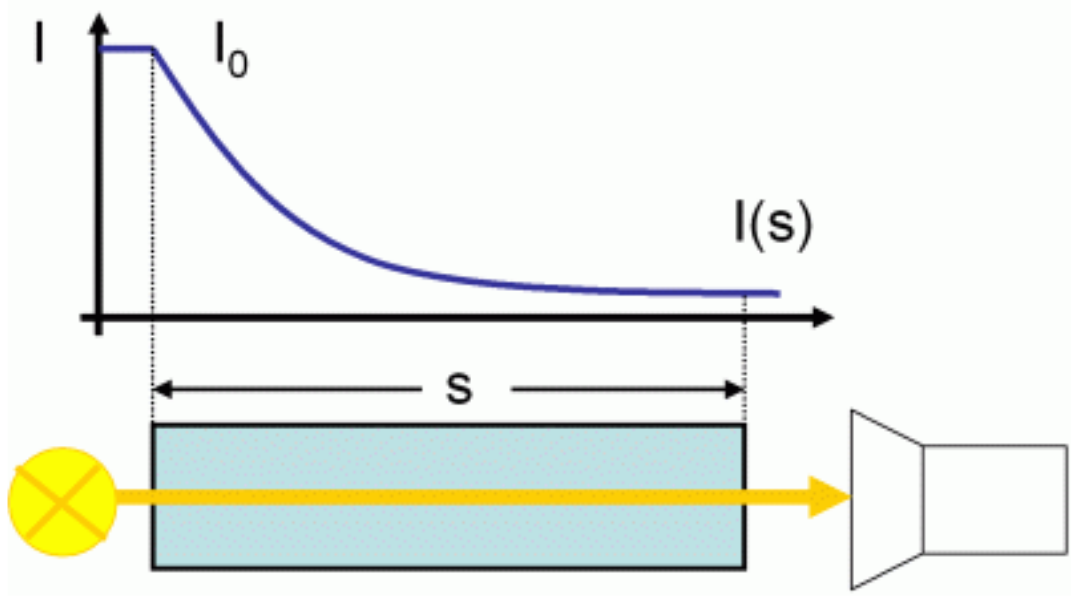
\includegraphics[width=55mm]{pic/lambert.png}
\hfil
\end{floatingfigure}
В однородной среде уменьшение интенсивности света в тонком слое
$ds$ пропорционально концентрации поглощающих молекул $\rho_{A}$,
их способности поглощать свет, сечению поглощения $\sigma_{A}$,
интенсивности $I$:
\begin{equation}
dI = - \rho_{A} \sigma_{A} I \, ds
\label{eq_Lambert}
\end{equation}
Интегрируя \eqref{eq_Lambert} приходим к экспоненциальному
уменьшению начальной интенсивности $I_{0}$ вдоль светового пути
$s$
\begin{equation}
I(s) = I_0 \exp(-\sigma_A \rho_A s)
\end{equation}
\textbf{Поглощение и рассеяние}
\nl
В атмосфере происходит не только поглощение, но и два типа
рассеяний: Рэлеевское рассеяние на частицах, 
малых по отношению к длине волны, и Ми-рассеяние на частицах, больших по отношению к длине волны.
Угасание света при рассеянии может быть рассмотрено так же, 
как и поглощение, используя сечения рассеяния $\sigma_{Ray}$ 
и $\sigma_{Mie}$. 
Зависимость рассеяния от длины волны $(\lambda)$ является 
гладкой и может быть аппроксимирована
полиномами: $\sigma_{Ray} \sim \lambda^{-4}$,
$\sigma_{Mie} \sim \lambda^{-1 \ldots +1}$.
\nl
Объединяя поглощение и рассеяние, мы получаем
\begin{equation}
I(s) =
I_0 \exp(
-\sigma_A \rho_A s \;
- \overbrace{\sigma_{Ray}}^{\substack{
\text{Сечение} \\ 
\text{релеевского} \\
\text{рассеяния}
}} \cdot
\underbrace{\rho_{Ray}}_{\substack{
\text{Концентрация} \\ 
\text{релеевских} \\ 
\text{рассеивателей}}} \cdot
s \;
- \;
\sigma_{Mie} \cdot \rho_{Mie} \cdot s
)
\end{equation}
В действительности существует не один поглотитель, а несколько.
Поглощения различных видов просто суммируется. 
Каждая молекула имеет характерный спектр поглощения с 
различной силой и специфической зависимостью от длины волны.
Включая несколько ($N$) поглотителей и явно показывая 
зависимость от длины волны, мы получаем:
\begin{equation}
I(s, \lambda) =
I_0(\lambda) \exp 
\left[
-\sum_{i=1}^N\sigma_{A_i} \rho_{A_i} s \;
- \sigma_{Ray} \cdot
\rho_{Ray} \cdot
s \;
- \;
\sigma_{Mie} \cdot \rho_{Mie} \cdot s 
\right]
\label{eq_sc}
\end{equation}
До сих пор мы предполагали однородную среду, но атмосфера 
таковой не является. 
Концентрация поглотителей сильно изменяется по высоте и по
горизонтали, поэтому мы вводим величину, называемую 
наклонное содержание $\text{SC}$, которая определяется 
как концентрация поглотителя, интегрированная вдоль пути света
\begin{equation}
SC_i = 
\int_{0}^{TOA}
\rho_{A_i} ds
\end{equation}
где $TOA$ -- верхняя часть атмосферы, предполагая, что 
прибор находится на земле.
\nl
Подставляя это в уравнение \eqref{eq_sc}, получаем
\begin{equation}
I(s, \lambda) =
I_0(\lambda) \exp 
\left[
-\sum_{i=1}^N\sigma_{A_i} \rho_{A_i} SC_i \;
- \sigma_{Ray} \cdot
\rho_{Ray} \cdot
SC_i \;
- \;
\sigma_{Mie} \cdot \rho_{Mie} \cdot SC_i 
\right]
\label{eq_sc_2}
\end{equation}
Как отмечалось ранее, сечения рассеяния пропорциональны полиномам
от длины волны, и поэтому могут быть аппроксимированы
\begin{equation}
\sigma_{Ray}(\lambda) \, SC_{Ray} +
\sigma_{Mie}(\lambda) \, SC_{Mie} =
\sum_{j=0}^{M} p_j \lambda^j   
\end{equation}
Подставляя это в уравнение \eqref{eq_sc_2}, получаем
\begin{equation}
I(s, \lambda) =
I_0(\lambda)
\exp
\left[
-\sum_{i=1}^N
\sigma_{A_i}(\lambda) \,
SC_i
- \sum_{j=0}^M
p_j \lambda^j
\right]
\end{equation}
Это уравнение можно преобразовать в линейное уравнение, 
взяв логарифм с обеих сторон, в результате чего получается
уравнение DOAS
\begin{equation}
\ln\underbrace{\dfrac{I(\lambda)}{I_0(\lambda)}}_{
\text{измерения}
} =
- \sum_{i=1}^N 
\overbrace{\sigma_{A_i}(\lambda)}^{
\substack{\text{известно} \\
\text{из} \\
\text{литературы}}}
\underbrace{SC_i}_{
\substack{
\text{что} \\
\text{мы} \\
\text{хотим} \\
\text{определить}
}
} +
\sum_{j=0}^{M} p_j \lambda^j
\end{equation}
Нам нужны два измерения($I$ и $I_0$): 
одно с поглощением, другое без него. 
Мы можем определить только интеграл количества поглотителя 
вдоль пути света (наклонных содержаний $SC_i$). 
В итоге имеем одно уравнение, но $N + M + 1$ неизвестных.
\nl
Поскольку уравнение DOAS должно выполняться для всех длин волн,
измерение на многих дискретных длинах волн 
$\lambda_1, \ldots, \lambda_k$  обеспечивает множество 
уравнений для одних и тех же $SC_i$ и $p_j$
\begin{equation}
\begin{split}
\ln \dfrac{I(\lambda_1)}{I_0(\lambda_1)} &=
- \sum_i \sigma_i(\lambda_1) SC_i +
\sum_{j} p_j \lambda_1^j \\
\ln \dfrac{I(\lambda_2)}{I_0(\lambda_2)} &=
- \sum_i \sigma_i(\lambda_2) SC_i +
\sum_{j} p_j \lambda_2^j \\
&\ldots \ldots \ldots \ldots \ldots \ldots \ldots \\
\ln \dfrac{I(\lambda_k)}{I_0(\lambda_k)} &=
- \sum_i \sigma_i(\lambda_k) SC_i +
\sum_{j} p_j \lambda_k^j
\end{split}
\end{equation}
Если $k$ достаточно велико, то это переопределенный набор
линейных уравнений, который можно решить с помощью 
стандартного линейного метода наименьших квадратов.
\nl
Эти уравнения независимы только в том случае, если сечения
поглощения достаточно сильно различаются как функции длины волны.
К счастью, сечение \no является очень хорошим кандидатом.
\nl
Всегда нужны два измерения: одно $I(\lambda)$ с поглотителем, 
а другое $I_0(\lambda)$ без поглотителя. 
К сожалению в атмосфере мы не можем удалить поглотитель.
\nl
Но нам достаточно иметь два измерения с разными путями 
света для решения этой проблемы:
\begin{equation}
\begin{cases}
\ln\dfrac{I_1(\lambda)}{I_0(\lambda)} &=
- \sum_i \sigma_i(\lambda) SC_{1, i} +
\sum_j p_j \lambda^j \\
\ln\dfrac{I_2(\lambda)}{I_0(\lambda)} &=
- \sum_i \sigma_i(\lambda) SC_{2, i} +
\sum_j p_j \lambda^j
\end{cases}
\end{equation}
Взятие разности снимает $I_0(\lambda)$
\begin{equation}
\ln \dfrac{I_1(\lambda)}{I_2(\lambda)} =
- \sum_i \sigma_i(\lambda)
(SC_{1, i} - SC_{2, i}) +
\sum_j p_j^* \lambda^j
\end{equation}
Как итоге DOAS основан на Законе Бугера--Ламберта--Бера. 
Следовые газы идентифицируются по характерной зависимости 
длины волны их спектров поглощения. 
Для одновременного измерения нескольких следовых газов 
необходимы измерения на многих длинах волн. 
Количество следовых газов определяется по величине поглощения.
Можно определить только общее количество следового газа,
интегрированное вдоль светового пути. 
Для анализа DOAS всегда требуется два измерения: текущее
измерение и эталонное измерение.
\nl
\textbf{MAX-DOAS \footnote{
2D MAX-DOAS -- если сканирование выполняется только по вертикали
(по углу места, elevation angle) при одном азимутальном
направлении визирования относительно солнца; \\
3D MAX-DOAS -- если сканирование выполняется как по углу места,
так и азимуту. \\
Мы рассматриваем 2D MAX-DOAS и обычно опускаем пояснение 2D.}} \\
\begin{figure}
\noindent\centering{
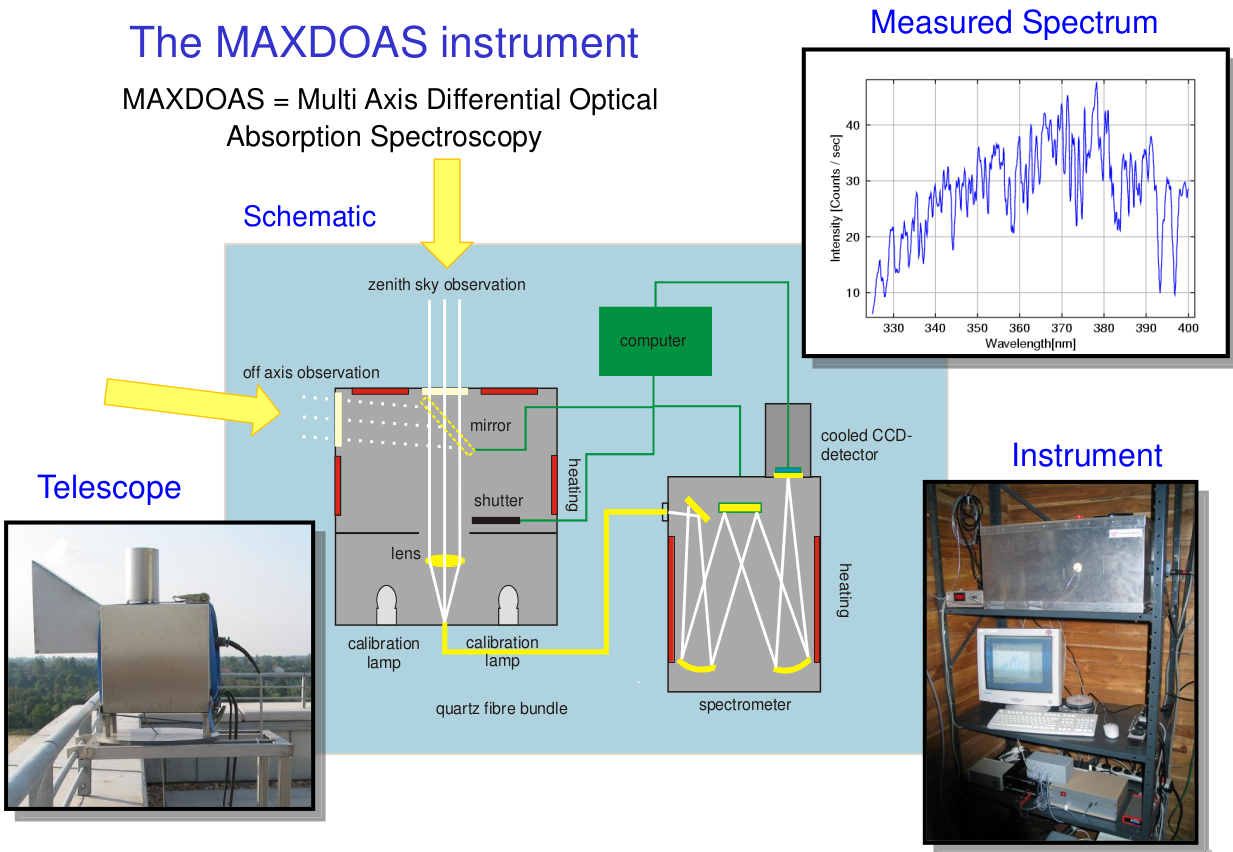
\includegraphics[width=110mm]{./pic/maxdoas.png}
}
\caption{Пример прибора MAX-DOAS}
\label{figCurves}
\end{figure}
Приборы DOAS часто делятся на две основные группы: пассивные 
и активные. 
Активные системы DOAS, такие как системы с длинным трактом(LP) 
и системы DOAS с усиленной полостью(CE), имеют собственный
источник света, тогда как пассивные используют солнце в качестве
источника света, например, MAX(Multi-axial)-DOAS. 
Луна также может быть использована для ночных измерений DOAS, 
но здесь обычно необходимо проводить измерения прямого света,
а не рассеянного, как в случае с пассивными системами DOAS,
такими как MAX-DOAS.
\nl
Телескоп для сбора света необходим для сбора  света из зенита
и с разных направлений над горизонтом. 
Сам телескоп находится на открытом воздухе, прибор в помещении.
Для передачи света от телескопа в лабораторию используется
волоконная оптика. 
Для измерения света на разных длинах волн используется
спектрометр. 
Для автоматизированного и количественного измерения детектор для
записи спектра.
\subsubsection{Понятие весовой функции и послойной воздушной массы}
Распространение света в атмосфере описывается
\textbf{интегральным уравнением переноса} относительно 
плотности столкновений фотонов $\rho = \rho(x)$ 
в фазовом пространстве $X$
\begin{equation}
\rho = K \rho + \psi
\end{equation}
где $\psi = \psi(x)$ -- плотность начальных столкновений,
$x=(r, \omega) \in X$ , $r$ -- радиус-вектор точки,
$\omega$ -- единичный вектор направления, 
$K$ -- интегральный оператор, 
ядро которого $k(x', x)$  является плотностью перехода 
фотона из точки $x'$ в точку $x$:
\begin{equation}
\int_X k(x', x) dx =
\dfrac{\sigma_S(r')}{\sigma(r')} \leq 1
\end{equation}
В частности, в том случае, когда фотон не попадает на 
поверхность планеты, ядро имеет вид
\begin{equation}
k(x', x) =
\dfrac{\sigma_S(r')}{\sigma(r')}
\cdot
\dfrac{
g(\mu, r') e^{-\tau(r', r) \sigma(r)}}{
2 \pi ||r - r'||^2}
\cdot
\delta(\omega - s) , \quad 
\mu = (s, \omega'),
s = \dfrac{1}{||r - r'||}(r - r')
\label{eq_kernel}
\end{equation}
где $\sigma_S(r)$ -- сечение рассеяния атмосферы в точке $r$,
$\sigma(r)$ -- полное сечение взаимодействия фотона со средой,
$g(\mu, r)$ -- нормированная на $1$ индикатриса рассеяния, 
$\delta(y)$ -- $\delta$-функция, 
$\tau(r', r) = \int_0^{||r-r'||}\sigma(r' + l \cdot s)$ --
оптическая длина отрезка $[r', r]$. 
При падении фотона на поверхность ядро $k(x', x)$ учитывает ее
отражающие свойства. 
Плотность начальных столкновений $\psi(x)$ зависит от плотности
распределения источников $s(x')$ как $\psi = Ks$, 
где интегральный оператор $K$ имеет ядро равное 
$k(x', x) = \dfrac{e^{- \tau(r', r) \sigma(r)}}{
||r - r'||^2
} \cdot \delta(\omega' - s) \cdot \delta(\omega - s)$.
\nl
Плотность столкновений $\rho(x)$ связана с решением 
\textbf{интегро - дифференциального уравнения переноса} --
плотностью потока или интенсивностью $I(x)$ -- равенством 
$\rho(x) = \sigma(r) I(x)$(если фотон несет единицу энергии).
\nl
В задачах дистанционного зондирования атмосферы можно
ограничиться оцениванием небольшого набора линейных функционалов 
$I_{\phi} = \int_X \phi(x) \rho(x) dx$ полного поля плотности
столкновений $\rho$, $\rho(x) \in \mathcal{L}_1$ -- пространство
абсолютно интегрируемых функций, 
$\phi(x) \in \mathcal{L}_{\infty}$ -- пространство ограниченных
почти всюду функций. Например, сигнал $I_*$ c приемника 
излучения $X_* = S_* \bigoplus \Omega_*$ объема $S_*$ и с полем
зрения $\Omega_*$ может быть получен при использовании функции
\begin{equation}
\phi_*(x) =
\dfrac{1}{\sigma (r)}
\delta_{\Omega_*}(\omega)
\delta_{S_*}(r) =
\dfrac{1}{\sigma (r)}
\delta_{X_*}(x)
\end{equation}
где $\delta_{\Omega_*}(\omega) = 1$ при 
$\omega \in \Omega_*$, $\delta_{\Omega_*}(\omega) = 0$
при $\omega \notin \Omega_*$ и
$\delta_{S_*}(r) = 1$ при $r \in S_*$,
$\delta_{S_*}(r) = 0$ при $r \notin S_*$ --
функции-индикаторы множеств $\Omega_*$ и $S_*$ соотвественно,
$\delta_{X_*}(x)=\delta_{\Omega_*}(\omega) \delta_{S_*}(r)$.
Действительно, для $I_*$ имеем
\begin{equation}
I_* = \int_{S_*} \int_{\Omega_*}
I(r, \omega) \, d\omega dr =
\int_{S_*} \dfrac{1}{\sigma (r)}
\int_{\Omega_*} \rho(r, \omega)
d \omega dr =
\left. I_{\phi} \right|_{\phi = \phi_*}
\end{equation}
Рассмотрим наряду с атмосферой с характеристиками, 
заданными ядром \eqref{eq_kernel}, возмущенную атмосферу, 
в которой сечение поглощения увеличено на величину 
$\triangle\sigma$ в области $R_+$. 
Ее характеристики будем помечать индексом $+$. 
Если $\delta_+(r)=1$, при $r \in R_+$, и 
$\delta_+(r)=0$ при $r \notin R_+$ -- 
функция-индикатор множества $R_+$, 
то сечения для возмущенной атмосферы имеют значения 
$\sigma_+(r) = \sigma(r) 
+ \triangle \sigma \cdot \delta_+(r)
, \sigma_{+S}(r) = \sigma_s(r)$.
\nl
В том случае, когда измеряется величина $I_\phi$,\\
\textbf{Весовой функцией} $w_\phi(R_+)$ области $R_+$ называется
\begin{equation}
w_q(R_+)=
\dfrac{dI_\phi}{d \sigma} =
\lim_{\triangle \sigma \rightarrow 0}
\dfrac{I_{+ \phi} - I_\phi}{\triangle \sigma}
\label{eq_weight_1}
\end{equation}
т.е. $w_\phi(R_+)$ есть производная $I_\phi$ по 
$\sigma(r)$, при $r \in R_+$. 
Для разности интенсивностей в возмущенной $I_{+ \phi}$ и
невозмущенной $I_{\phi}$ атмосферах имеем:
\begin{equation}
I_{+ \phi} - I_\phi = 
\triangle \sigma \cdot w_\phi (R_+) +
\sigma(\triangle \sigma)
\end{equation} 
В тех случаях, когда рассматривается сферически симметричная или
плоскопараллельная атмосфера и область $R_+$ является слоем
толщиной $L_+$, имеет смысл ввести понятие эффективной воздушной
массы слоя $R_+$ для наблюдаемого параметра $I_\phi$. 
\textbf{Эффективная воздушная масса слоя} атмосферы 
$R_+$ равна среднему пробегу в слое $R_+$ фотонов, попадающих 
на приемник излучения, отнормированному на толщину слоя $L_+$. 
Для детектора, расположенного вне слоя $R_+$, имеем равенство,
связывающее весовые функции с эффективной воздушной массой слоя:
\begin{equation}
w_\phi(R_+) =
-L_+ \cdot m_\phi(R_+) \cdot I_\phi
\label{eq_weight_2}
\end{equation}
Введенное понятие эффективной воздушной массы слоя атмосферы 
для рассеянного излучения аналогично понятию воздушной массы,
вводимому при рассмотрении прямого излучения. 
Согласно закону Бугера ослабление солнечного излучения 
атмосферой в плоскопараллельном приближении описывается
выражением:
\begin{equation}
I^p = I_0^p \exp \left[
-m \sum_i s_i \int c_i(h) dh
\right]
\end{equation}
где $I^p$ -- интенсивность прошедшего атмосферу излучения,
$I_0^p$ -- внеатмосферная интенсивность, $s_i$ -- сечение
поглощения газа с концентрацией $c_i(h)$, 
$m=1/\cos(z)$ -- так называемая воздушная масса атмосферы при
зенитном угле солнца $Z$. Коэффициент $m$ равен отношению
оптической толщи атмосферы при ее наклонном прохождении под 
углом $Z$ к толще при прохождении по нормали.
Интенсивность в возмущенной атмосфере $I_+^p$ с концентрацией
газов $c_i(h)+\triangle c_i(h)$ будет равна
\begin{equation}
I_+^p = I^p
\exp\left[
-m\sum_i s_i \int \triangle c_i(h) dh
\right]
\label{buger}
\end{equation}
Для прямого излучения в сферической атмосфере аналогично
получаем:
\begin{equation}
I_+^s =
I^s \exp \left[
- \int m(h) \sum_i
s_i \triangle c_i (h) dh
\right]
\label{eq_IplusS}
\end{equation}
где $m(h) = 1 / \cos(z(h))$, $z(h)$ -- угол пересечения слоя
светом. 
Коэффициентh $m()$ для слоя на высоте $h$ имеет тот же смысл, 
что и $m$ для всей атмосферы в выражении \eqref{buger}.
\nl
Понятие воздушной массы слоя введем для приближения сферической
симметричной атмосферы. 
Данное приближение используется только для рассмотрения аналогии
воздушных масс прямого и рассеянного излучения, но не
распространяется на результаты, полученные для вычисления 
весовых функций. 
Для возмущения в одном слое из равенств \eqref{eq_weight_1} 
и \eqref{eq_weight_2}, находим: 
$I_{+ \phi} = I_\phi + w_\phi(R_+) \cdot \triangle
\sigma + o(\triangle \sigma) =
I_\phi \cdot (1 - L_+ \cdot m_\phi (R_+) \cdot \triangle
\sigma) + o(\triangle \sigma)=
I_\phi \exp(-L_+ \cdot m_\phi(R_+) \cdot \triangle \sigma) +
o(\triangle \sigma)$. А для возмущения во всей атмосфере соответственно:
\begin{equation}
I_+ = 
I \exp\left[
- \int m(h) \sum_i s_i \triangle c_i(h) dh
\right]
+ o(||\triangle c||)
\label{eq_Iplus}
\end{equation}
С точностью до малого члена $o(||\triangle c||)$ представление
\eqref{eq_Iplus} эквивалентно равенству \eqref{eq_IplusS}, 
связывающему прямое (ослабленное атмосферой) солнечное излучение
в возмущенной и невозмущенной атмосферах. 
По аналогии с прямым солнечным излучением имеет смысл назвать
$m(h)$  эффективной воздушной массой слоя атмосферы, 
лежащего на высоте $h$, для данного вида наблюдений и 
оптического состояния атмосферы. 
Величина воздушной массы слоя атмосферы показывает, во сколько
раз по сравнению с геометрической толщиной слоя эффективно
увеличивается путь света за счет наклонного и многократного
прохождения слоя. 
Как и воздушная масса для прямого излучения, эффективная
воздушная масса слоя для рассеянного излучения будет одинакова
для всех газов на выбранной длине волны. 
Однако, в отличие от воздушной массы слоя для прямого излучения,
которая полностью определяется углом прохождения света сквозь
слой $z(h)$, эффективная воздушная масса (ВМ) слоя (ВМ) зависит
не только от направления наблюдения и положения Солнца, 
но также от всех оптических характеристик атмосферы и
подстилающей поверхности. 
Для нашей задачи в дальнейшем важно то, что эффективная ВМ слоя
зависит от аэрозоля.
\subsubsection{Схема зенитных спектральных наблюдений}
Измеряется солнечная радиация, приходящая из ряда направлений: 
от зенита до горизонта. 
Измерения производятся при заданном угле Солнца, 
за время измерений Солнце практически не сдвигается
см на Рис. \ref{pic:scheme}.
Метод DOAS позволяет определить содержания примесей в 
наклонном столбе атмосферы $\xi(\theta_i)$ 
для всех зенитных углов солнца $\theta_i$:
\[
\xi(\theta_i) = 
\int_0^H
m(h, \theta_i) n(h) dh
\]где $m(h, \theta_i)$ -- 
послойная воздушная масса, 
которая рассчитывается из модели
переноса излучения. 
Она связывает наклонное содержание $\text{NO}_2$ 
$\xi(\theta)$ 
с вертикальным распределением концентраций $n(h)$. 
Недостатком этого метода является сложность в интерпретации
полученных непосредственно из спектров, 
наклонных содержаний микропримесей, сложности моделирования
переноса излучения, что необходимо для решения обратной 
задачи (задачи нахождения коэффициентов пропорциональности 
между наклонными и общими содержаниями микропримесей).
\begin{figure}[h]
\noindent\centering{
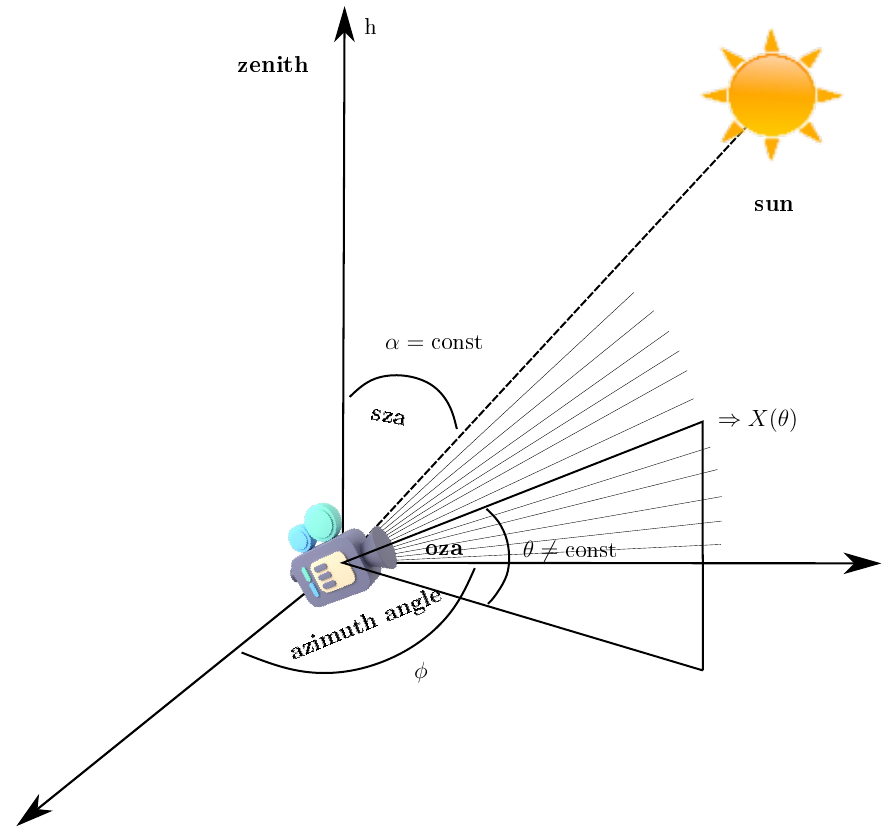
\includegraphics[width=110mm]{./pic/scheme.png}
}
\caption{Схема зенитных спектральных наблюдений}
\label{pic:scheme}
\end{figure}
\clearpage
\section{Предложенный метод}
\subsection{Линейное программирование}
В задачах линейного программирования требуется минимизировать
линейную функцию на множестве, заданном как решение системы
линейных уравнений или неравенств. 
Линейное программирование 
-- это частный случай математического программирования.
\nl
Основной задачей линейного программирования называется задача
нахождения минимума линейной целевой функции:
\begin{equation}
\max\limits_{\pmb x} \, 
(\pmb c^T \pmb x \, | \, \pmb x \in \mathbb{R}^n
\, \wedge \, A \pmb x \leq \pmb b \, \wedge \, \pmb x \geq 0)
\end{equation}
где $\pmb x$ -- вектор, который необходимо определить,
$\pmb c$, $\pmb b$ и $A$ -- заданные векторы и заданная
матрица соотвественно.
Неравенства $A \pmb x \leq b$ и $\pmb x \geq 0$ являются
ограничениями, задающими выпуклый многогранник, по которому
должна быть оптимизирована целевая функция.
\nl
Каждая задача линейного программирования(основная задача), 
может быть преобразована в двойственную задачу, 
которая обеспечивает  верхнюю границу оптимального 
значения основной задачи. 
В матричной форме мы можем выразить основную задачу как:
\begin{multline}
\max\limits_{\pmb x} \, 
(\pmb c^T \pmb x \, | \, \pmb x \in \mathbb{R}^n
\, \wedge \, A \pmb x \leq \pmb b \, \wedge \, \pmb x \geq 0)
\; \Leftrightarrow \\
\Leftrightarrow \;
\max\limits_{\pmb y} \, 
(\pmb b^T \pmb y \, | \, \pmb y \in \mathbb{R}^n
\, \wedge \, A^T \pmb y \geq \pmb b \, \wedge \, \pmb y \geq 0)
\end{multline}
Любая задача ЛП сводится к канонической:
\begin{equation}
\max\limits_{\pmb x} \, 
(\pmb c^T \pmb x \, | \, \pmb x \in \mathbb{R}^n
\, \wedge \, A \pmb x = \pmb b \, \wedge \, \pmb x \geq 0)
\end{equation}
Алгоритм перехода от произвольной задачи ЛП к канонической форме:
\begin{enumerate}
\item Неравенства с отрицательными $b_i$ 
умножаются на $(-1)$.
\item К левой части прибавляются $s_i$.
\footnote{Нумеруем $s_i$ по номеру неравенства, 
в которое мы его добавили.
\label{note:s1}}
\footnote{$s_i \geq 0$.
\label{note:s2}} -- добавочную переменную, 
и получаем равенство.
\item Делаем замену переменных:
\begin{itemize}
\item Если $x_i \leq 0$, то $x_i'= -x_i \geq 0$.
\item Если $x_i$ — любой, то $x_i= x_i' - x_i''$, где 
$x_i', x_i''\geq 0$.
\end{itemize}
\end{enumerate}
\subsubsection{Симплекс метод}
Введём некоторые определения:
\nl
\textbf{Допустимое решение} -- это любое неотрицательное 
решение системы ограничений. 
\nl
Пусть имеется система $m$ ограничений с $n$ переменными 
$(m < n)$.
\textbf{Допустимое базисное решение} --  это решение, 
содержащее $m$ неотрицательных \textbf{основных(базисных)}
переменных и $n - m$ неосновных(\textbf{свободных}) переменных.
\nl 
Неосновные переменные в базисном решении равны нулю, 
основные же переменные, как правило, отличны от нуля, 
то есть являются положительными числами.
\nl
Любые $m$ переменных системы $m$ линейных уравнений с 
$n$ переменными называются основными, если определитель 
из коэффициентов при них отличен от нуля. 
Тогда остальные $n - m$ переменных называются неосновными.
\nl
Алгоритм симплекс метода:
\begin{description}
\item[I.] . Приводим задачу линейного программирования к
канонической форме.
\item[II.] Если в полученной системе $m$ уравнений, 
то $m$ переменных принимаем за основные. 
Далее выражаем основные переменные через неосновные и 
находим соответствующее базисное решение. 
Если найденное базисное решение окажется допустимым, 
необходимо перейти к допустимому базисному решению.
\item[III.] Выражаем функцию цели через неосновные переменные
допустимого базисного решения. 
Если отыскивается максимум (минимум) линейной формы, 
и в её выражении нет неосновных переменных с
отрицательными(положительными) коэффициентами,
то критерий оптимальности выполнен, 
и полученное базисное 
решение является оптимальным. 
Если при нахождении максимума(минимума) линейной формы в её
выражении имеется одна или несколько неосновных переменных с
отрицательными(положительными) коэффициентами, переходим к 
новому базисному решению
\end{description}
\subsection{Сведение обратной задачи к задаче линейного программирования}
Часто при решении уравнений вида
\begin{equation}
\pmb\xi = M \pmb n
\label{eq:inverse_prob}
\end{equation}
, где $\pmb n$ и $\pmb\xi$ -- векторы линейных 
пространств размерности $d_1$ и $d_2$ соответственно, 
а $M$ -- линейный оператор, вместо решения уравнения
\eqref{eq:inverse_prob} проще найти такой вектор $n$, 
при котором $Mn$ как можно ближе к $\pmb\xi $ в метрике
пространства $C$ с нормой
$||\pmb \xi|| = \max_{i=1, \ldots, d_2} |\xi_i|$.
\nl
Пусть линейный оператор задан матрицей $||m^p_k||^{d_2}_{d_1}$, 
строки которой обозначим 
$m_i, \, i = \overline{1, d_2}$. $\pmb \xi$ соотвествует
$||\xi^p||^{d_2}$, $\pmb n$ соотвествует $||n^p||^{d_1}$.
Тогда уравнение \eqref{eq:inverse_prob} примет вид:
\begin{equation}
\xi_i = (m_i^T, \pmb n), 
\quad i = \overline{1, d_2}
\end{equation}
Вместо решения системы уравнений \eqref{eq:inverse_prob}
рассмотрим задачу на минимакс
\begin{equation}
\min_{\pmb n}\max_{i=\overline{1, d_2}} 
|\xi_i - (m_i^T, \pmb n)|
\end{equation}
Эта задача на минимакс сводится к задаче линейного
программирования. 
\nl
Действительно, для вычисления модуля $|d|$
требуется найти минимальное из чисел $z$, для которых 
выполнены неравенества $|d| = \min_{z} \{ z \, | \, z 
\geq d \wedge z \geq -d\}$.
\nl
Соответственно:
\begin{equation}
\max_{i=\overline{1, d_2}} |\xi_i - (m_i^T, \pmb n)| = 
\min_{z} \{z \,| \, z \geq \xi_i - (m_i^T, \pmb n) 
\wedge z \geq -\xi_i + (m_i^T, \pmb n)\}
, \quad i = \overline{1, d_2}
\end{equation}
Введём два вектора 
$s = (z, n_1, \ldots, n_{d_1})$ и $t = (1, 0, \ldots, 0)$. \\
Их скалярное произведение$(s, t) = z$.
Минимизация по $s$ при наложенных ограничениях даст нам
решение искомой задачи:
\begin{equation}
\min_s \{(s, t) \, | \,  z \geq \xi_i - (m_i^T, \pmb n) 
\wedge z \geq -\xi_i + (m_i^T, \pmb n)\}
, \, i = \overline{1, d_2} \}\, \Longrightarrow \, s
\label{eq:minimize}
\end{equation}
\subsubsection{Априорная информация о профиле}
В дополнение к вышесказанному необходимо учитывать наличие 
априорной информации о профиле:
\begin{description}
\item[I.] Случай одного максимума и неотрицательность
концентраций
$$\exists c \in {1, \ldots, d_1}:
\begin{cases}
n_1 \leq n_2, \\
\ldots \\
n_{c-1} \leq n_{c}, \\
n_{c} \geq n_{c+1}, \\
\ldots \\
n_{d_1 - 1} \geq n_{d_1}.
\end{cases}
\qquad \wedge \qquad \forall i \;  (n_i \geq 0).$$
$c$ перебором выбирается таким образом, чтобы выражение
\eqref{eq:minimize} было минимально.
\item[II.] Случай двух максимумов и 
неотрицательность концентраций
$$\exists c_1, c_2, c_3 \in {1, \ldots, d_1}:
\begin{cases}
n_1 \leq n_2, \\
\ldots \\
n_{c_1-1} \leq n_{c_1}, \\
n_{c_1} \geq n_{c_1+1}, \\
\ldots \\
n_{c_2-1} \geq n_{c_2}, \\
n_{c_2} \leq n_{c_2+1}, \\
\ldots \\
n_{c_3-1} \leq n_{c_3}, \\
n_{c_3} \geq n_{c_3+1}, \\
\ldots \\
n_{d_1 - 1} \geq n_{d_1}.
\end{cases}
\qquad \wedge \qquad \forall i \;  (n_i \geq 0).$$ 
\end{description}
$c_1, c_2, c_3$ перебором выбирается таким образом, 
чтобы выражение \eqref{eq:minimize} было минимально.
\subsubsection{Проверка адекватности}
Проверить согласие предположения об унимодальности профиля
концентрации \no с результатом измерения можно, если известны
ограничения на координаты $\nu_i$ погрешности измерения. 
Если $|\nu_i| \leq \epsilon_i$, то полученный минимизацией
по $c_1$ задачи \eqref{eq:minimize} профиль не противоречит
результату измерения, если значение минимума \eqref{eq:minimize}
не больше, чем $\epsilon$.
\nl 
Если же это условие не выполнено, можно усложнить модель, 
считая, что профиль концентрации имеет два максимума и один
минимум.
\section{Эксперименты}
\subsection{Подготовка}
\subsubsection{Послойные воздушные массы}
Послойные воздушные массы $m(h_i, \theta_j)$
получаются решением задачи переноса излучения в атмосфере 
методом Монте-Карло, для этого использовалась математическое
обеспечение, созданное в 
Институте физики атмосферы имени А. М. Обухова РАН.
\nl
Расчёты выполнялись при szas=$60^{\circ}$,  
saas= $0^{\circ}$,  
$\lambda_{NM}$= $450$,  
albedo= $0.05$. 
Зенитные углы направления визирования $\theta_j$ 
выбирались исходя из исследований \cite{litlink4}, 
в которых было показано, что максимальный
вклад в формировании $m(h_i, \theta_j)$ вносят углы 
близкие к $90^{\circ}$. 
И сетка для : oza = $[$ $0.0^{\circ}$, $10.0^{\circ}$,
$20.0^{\circ}$, $30.0^{\circ}$, $40.0^{\circ}$, $50.0^{\circ}$,
$60.0^{\circ}$, $70.0^{\circ}$, $75.0^{\circ}$, $80.0^{\circ}$,
$82.0^{\circ}$, $84.0^{\circ}$, $85.0^{\circ}$, $86.0^{\circ}$,
$87.0^{\circ}$, $88.0^{\circ}$, $89.0^{\circ}$, $89.3^{\circ}$,
$89.6^{\circ}$, $89.8^{\circ}$, $89.9^{\circ}$ $]$.
\begin{figure}[bh]
\noindent\centering{
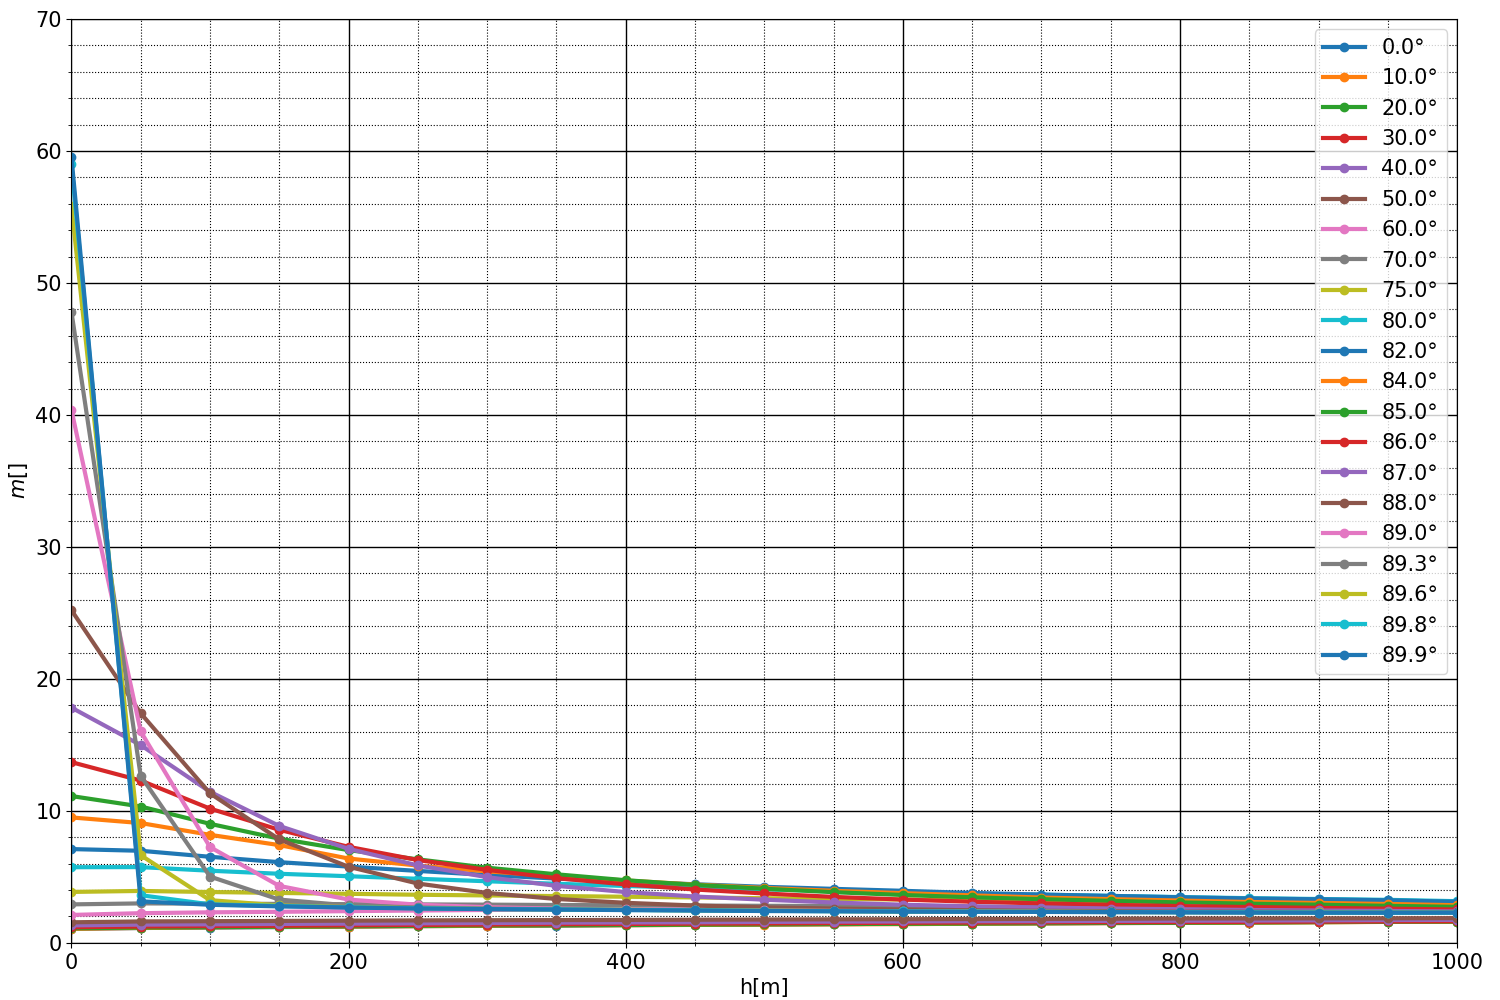
\includegraphics[width=155mm]{./pic/Figure_1.png}
}
\caption{Послойные воздушные массы для различных
углов направления визирования.}
\label{weights}
\end{figure}  

Сетка высот  также выбиралась следующим образом:
\begin{itemize}
\item для высот от $0$ до $4$ км: $\triangle h$ = $0.05$ км,
\item для высот от $4$ до $45$ км: $\triangle h$ = $1$ км, 
\item для высот от $45$ км до $85$ км: $\triangle h$ = $5$ км. 
\end{itemize}
Данный выбор сетки обосновывается тем, что на больших высотах
методы расчёта послойных воздушных масс не позволяют определять
точно профили газов \cite{litlink3}. 
\nl
На Рис. \ref{weights} изображены зависимости послойных воздушных 
масс от высоты для разных направлений визирования.
\nl
\subsubsection{Профили}
Для проверки эффективности описанного метода были проведены
модельные эксперименты по измерению содержания \no  в 
атмосфере. 
Источником основы профилей, изображённых на 
Рис. \ref{pic:prof_original} служат данные прямых измерений
\no в различные временные промежутки \cite{litlink4}
\begin{figure}[bh]
\noindent\centering{
\noindent
\begin{center}
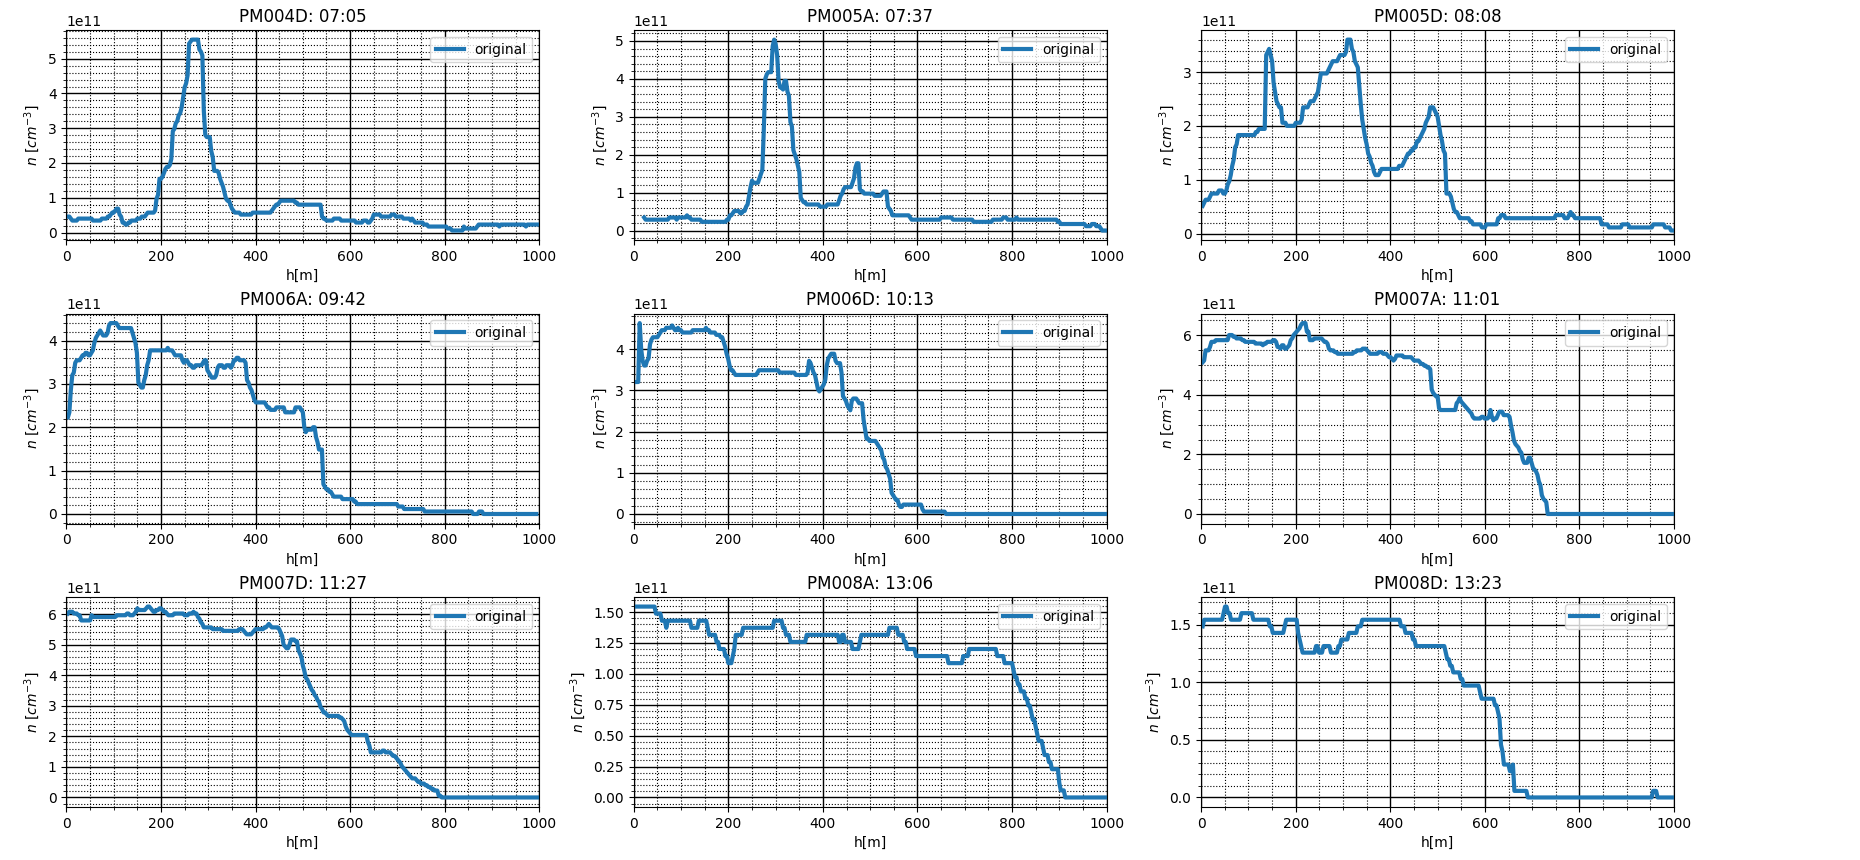
\includegraphics[width=165mm]{./pic/proforig_1.png}
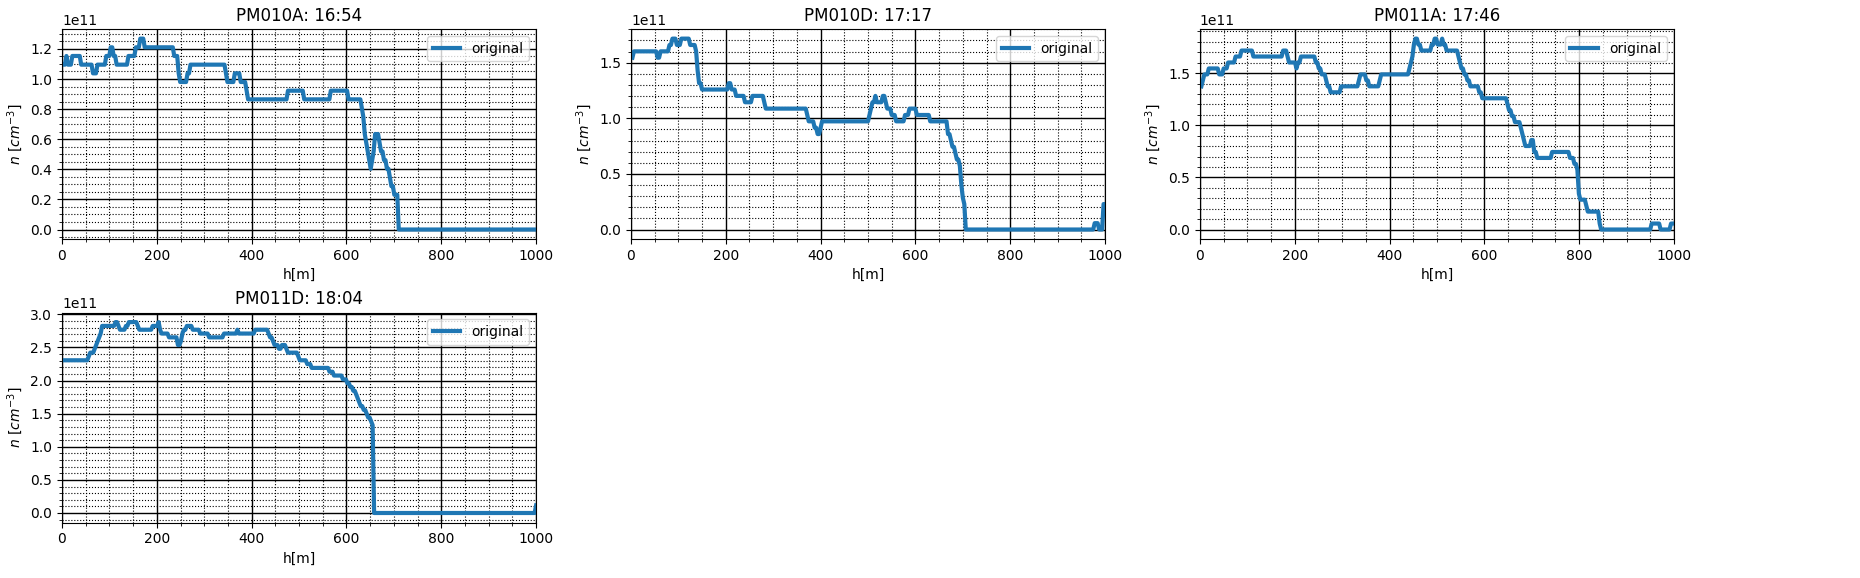
\includegraphics[width=165mm]{./pic/proforig_2.png}
\end{center}
\label{pic:prof_original}
\caption{Концентрация $\text{NO}_2$ в атмосфере
измеренные в течения дня \cite{litlink4}}
}
\end{figure}
\subsubsection{Прямые измерения}
Далее рассчитывается наклонное содержание \no :
\begin{multline}
\xi_j = \xi(\theta_j) = \int_{0}^{H} m(\theta_j, h) 
\cdot n(h) \, dh 
+ \nu_j = \\
= \sum_{i=0}^{N-1} \left[
m \left(\theta_j, \frac{h_{i+1} - h_i}{2} \right) 
\cdot 
\dfrac{\int^{h_{i+1}}_{h_i} n(h)}{h_{i+1} - h_i}) \, 
\triangle h_i \right]
+ \nu_j
\label{eq:direct_measurment}
\end{multline}

Где $\nu_j$ согласно \cite{litlink6}
представлена в двух вариантах: 
$\nu_j \sim \mathcal{N}(0, (0.1 * 10^{15})^2)$ и
$\nu_j \sim \mathcal{N}(0, (0.3 * 10^{15})^2)$.
\begin{figure}[h]
\noindent\centering{
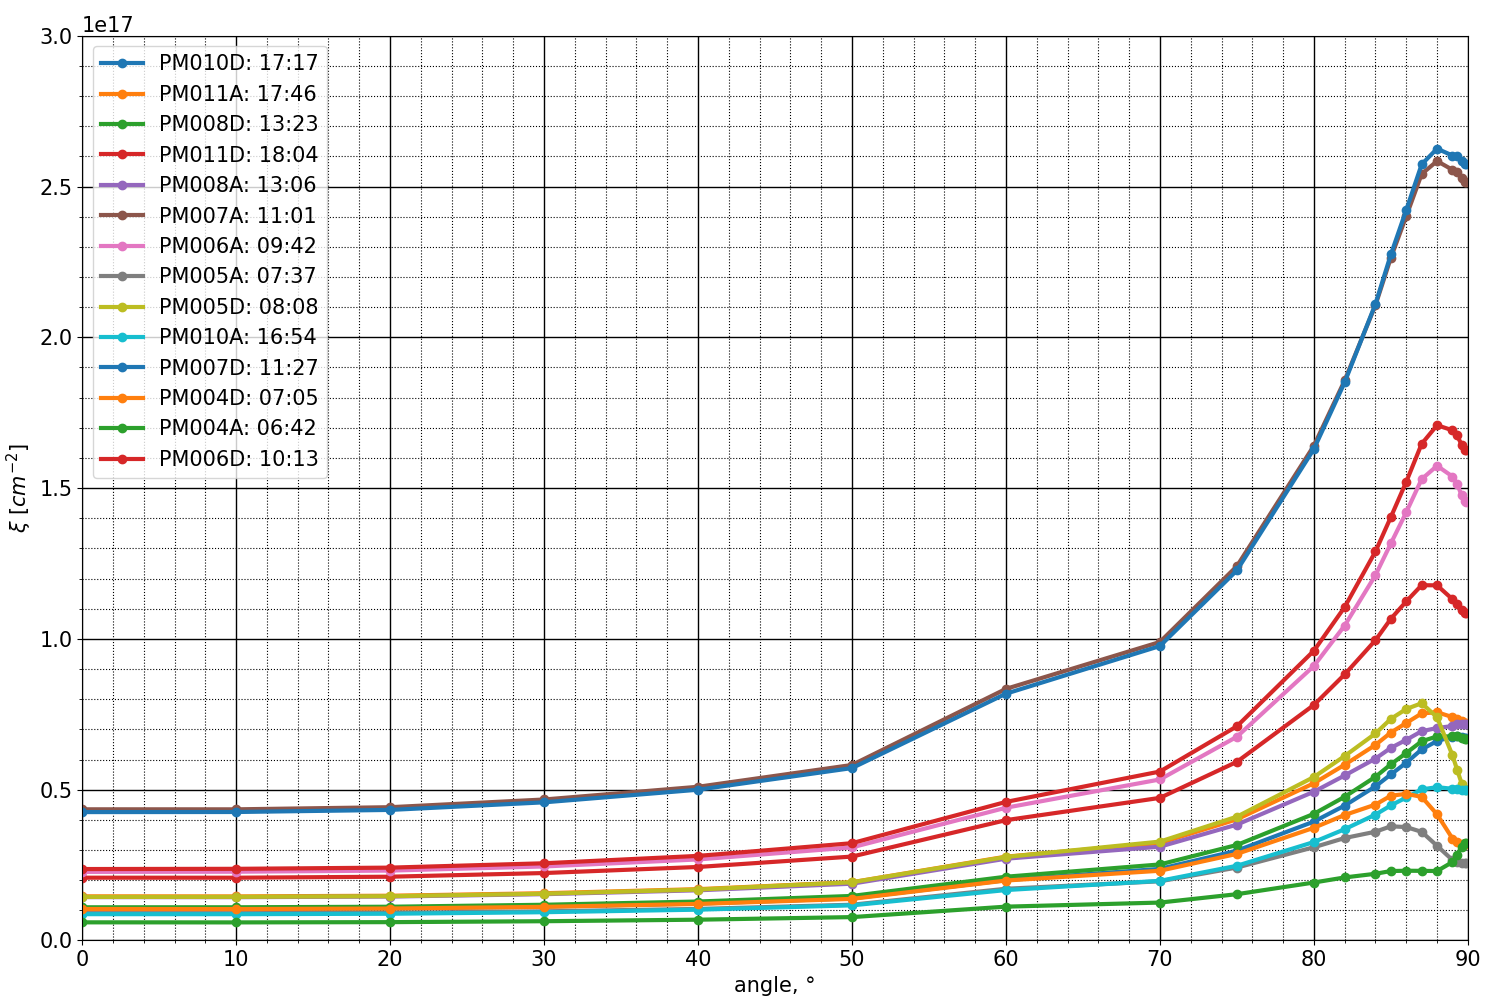
\includegraphics[width=155mm]{./pic/slant_no2.png}
\label{pic:direct_measurment}
\caption{Наклонные содержания $\text{NO}_2$ профилей
\ref{pic:prof_original} в атмосфере рассчитанные по 
\eqref{eq:direct_measurment} при $\nu_j = 0$, $\text{szas}=60^{\circ}, \lambda_{NM}= 450\text{нм},
\text{albedo}=0.05$.}}
\end{figure}
\clearpage
\begin{figure}[h]
\noindent\centering{
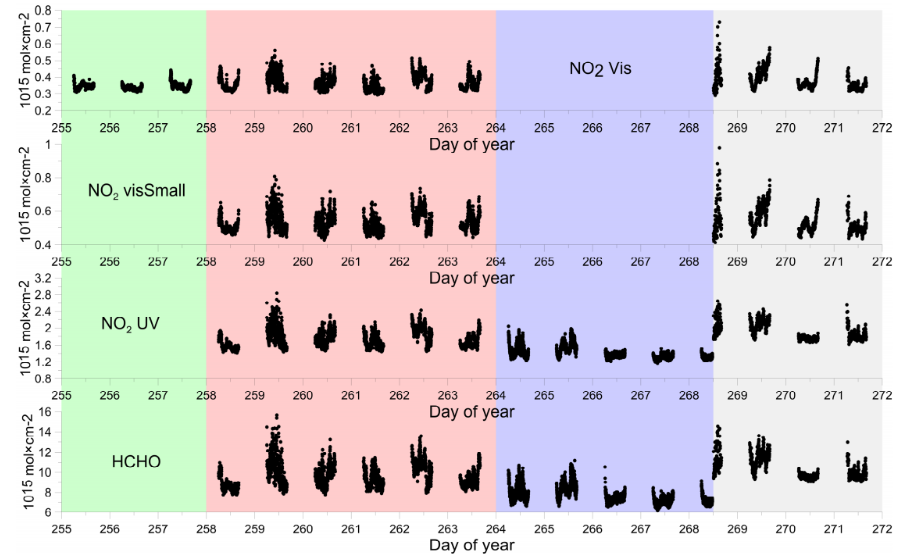
\includegraphics[width=155mm]{./pic/slant_error.png}
\label{pic:direct_measurment}
\caption{Ошибки при измерении наклонного содержания 
$\text{NO}_2$ профилей \ref{pic:prof_original} в атмосфере
рассчитанные из \cite{litlink6}}}
\end{figure}
\subsection{Результаты восстановления}
Для решения задачи линейного программирования
использовался симплекс метод из пакета $SciPy$.
На Рис. \ref{prof_12}, \ref{prof3_12},
\ref{proff_12}, \ref{proff3_12} голубая гистограмма --
оригинальный профиль(
$\frac{\int_{h_{i}}^{h_{i+1}} n(h) \, dh}{
h_{i+1} - h_i} , \; i=\overline{1, N-1}$), 
красная гистограмма -- один восстановленный профиль,
чёрный error bar -- усреднение $30$-ти восстановленных профилей
со стандартным отклонением в качестве ошибки.
\clearpage
\subsubsection{I случай(один максимум)}
\begin{figure}[bh]
\noindent\centering{
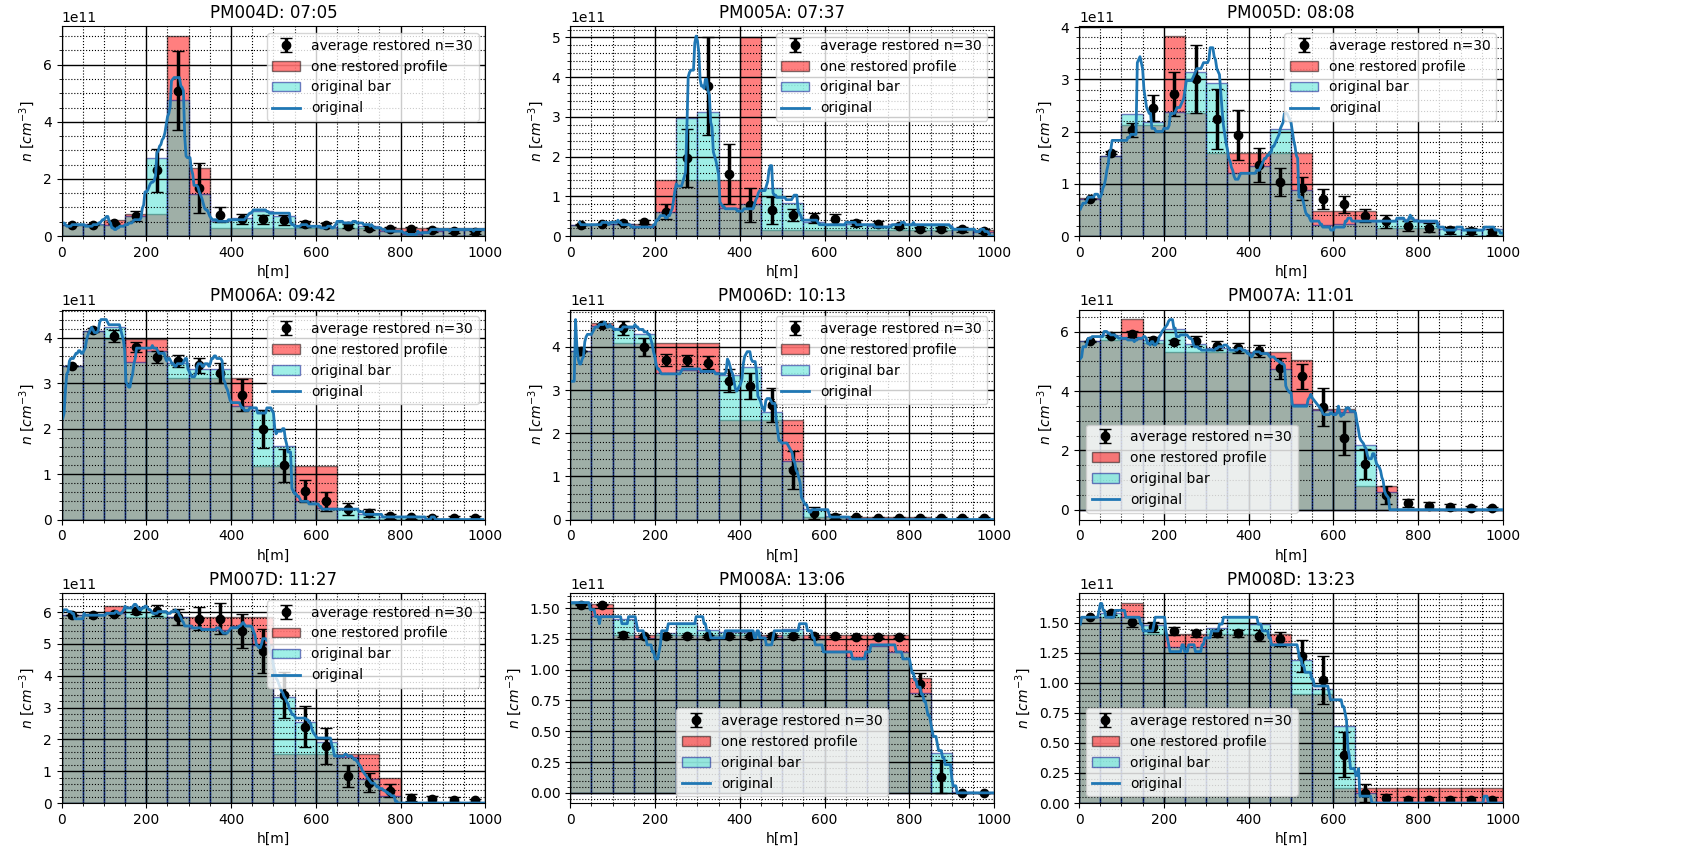
\includegraphics[width=180mm]{./pic/prof_1.png}
\noindent
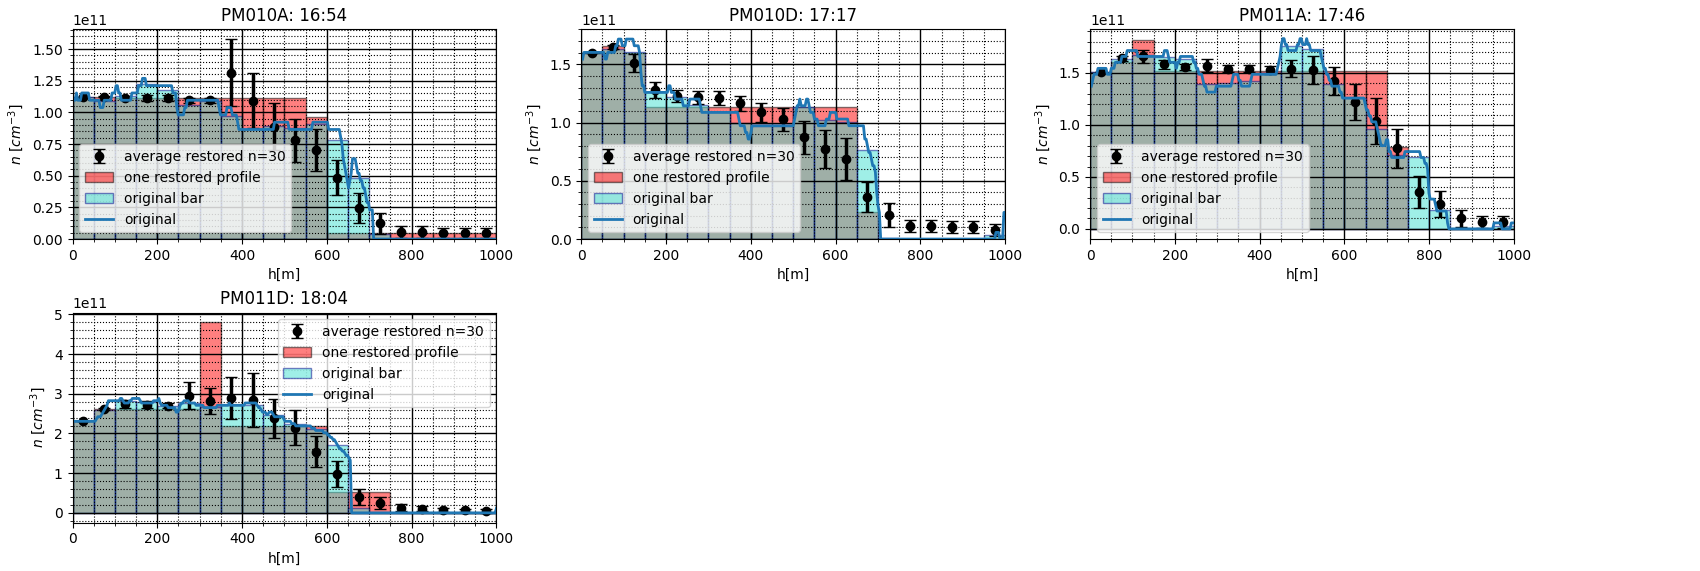
\includegraphics[width=180mm]{./pic/prof_2.png}
}
\caption{Результаты восстановления профилей при
$\text{szas}=60^{\circ}, \lambda_{NM}= 450\text{нм},
\text{albedo}=0.05, \nu_j \sim 
\mathcal{N}(0, (0.1 * 10^{15})^2)$.}
\label{prof_12}
\end{figure}
\newpage
\begin{figure}[bh]
\noindent\centering{
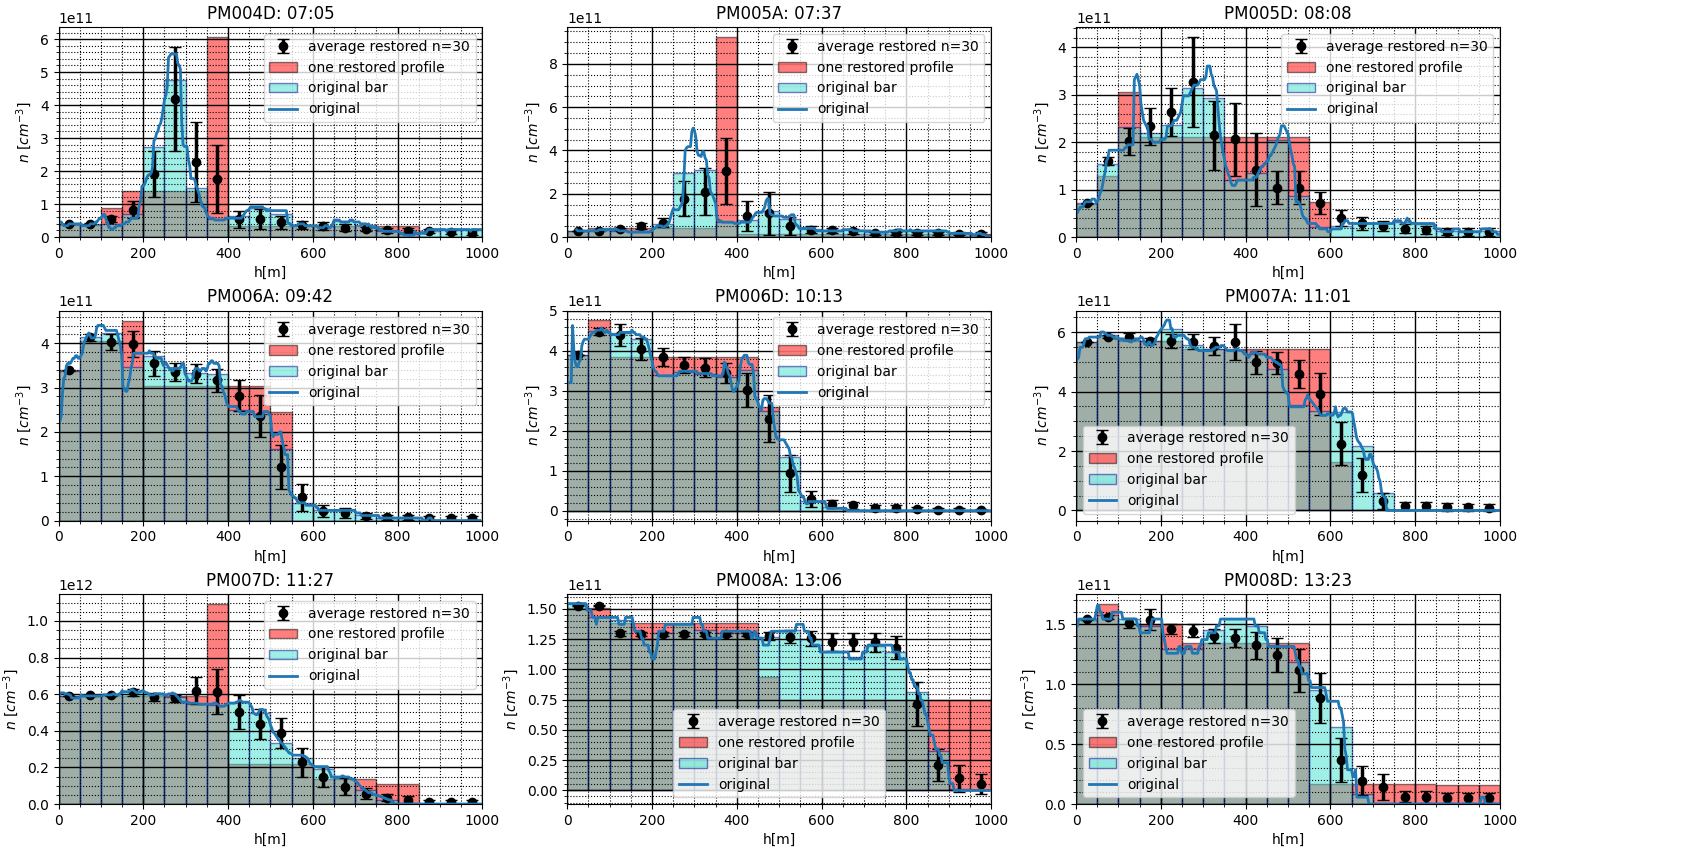
\includegraphics[width=180mm]{./pic/prof3_1.png}
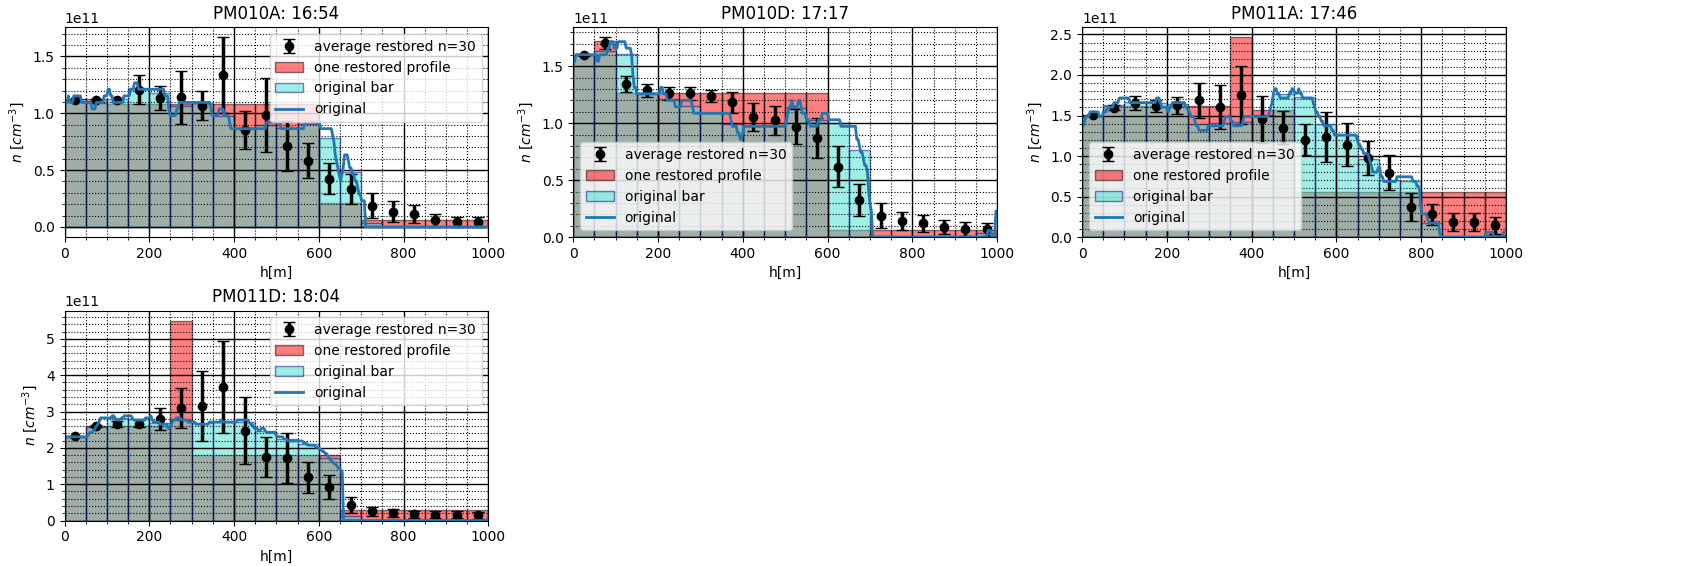
\includegraphics[width=180mm]{./pic/prof3_2.png}
}
\caption{Результаты восстановления профилей при
$\text{szas}=60^{\circ}, \lambda_{NM}= 450\text{нм},
\text{albedo}=0.05, \nu_j \sim 
\mathcal{N}(0, (0.3 * 10^{15})^2)$.}
\label{prof3_12}
\end{figure}
\clearpage
\subsubsection{II случай(два максимума)}
\begin{figure}[bh]
\noindent\centering{
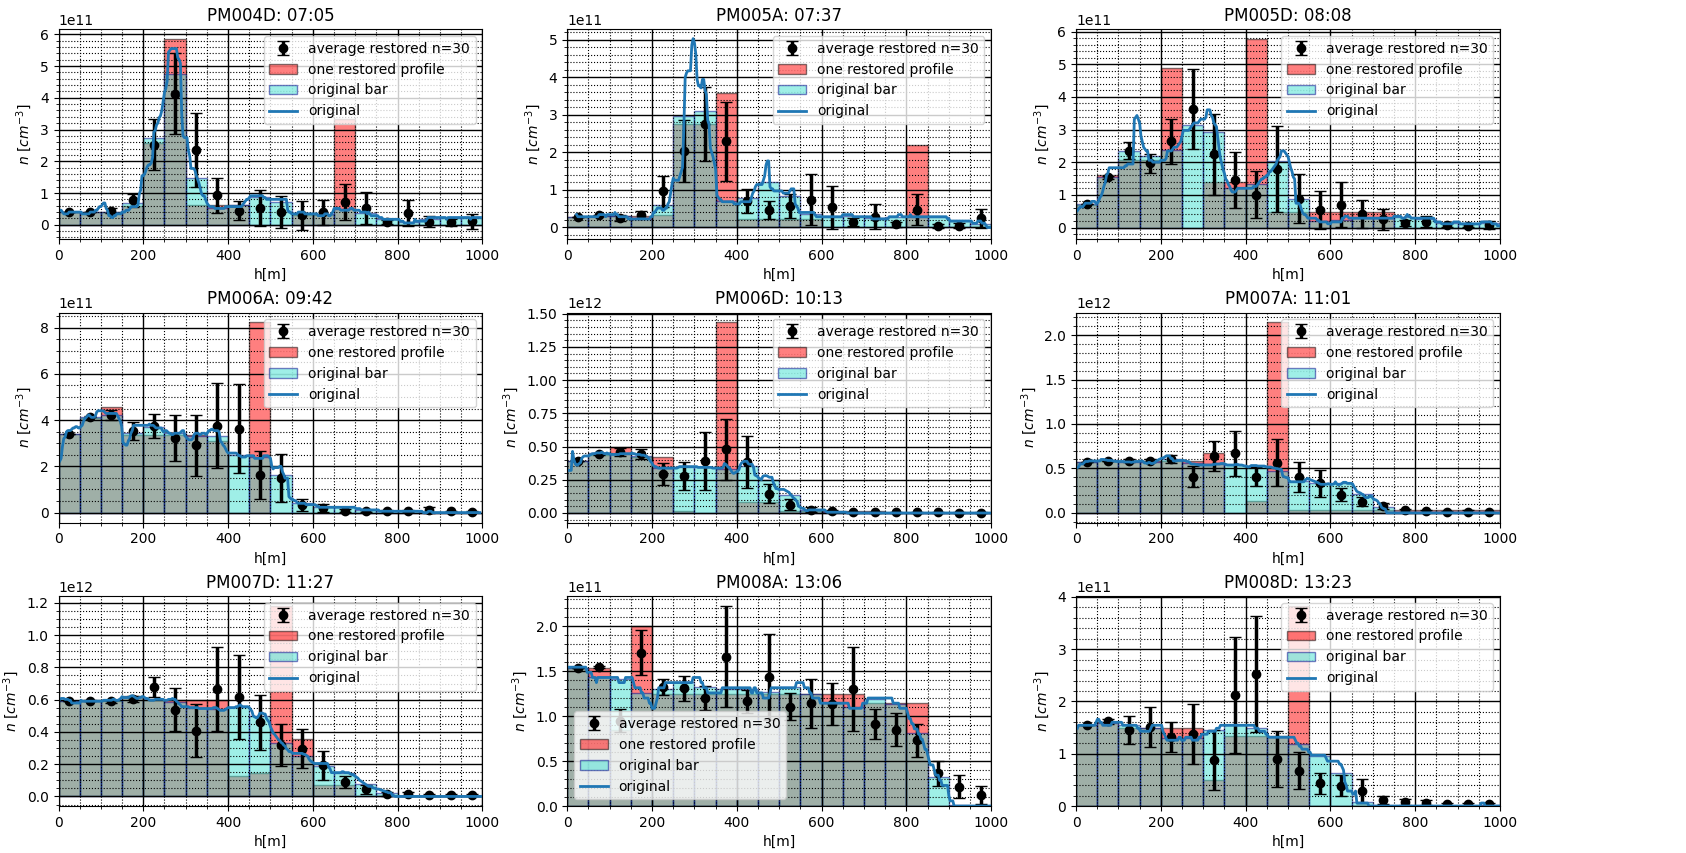
\includegraphics[width=180mm]{./pic/proff_1.png}
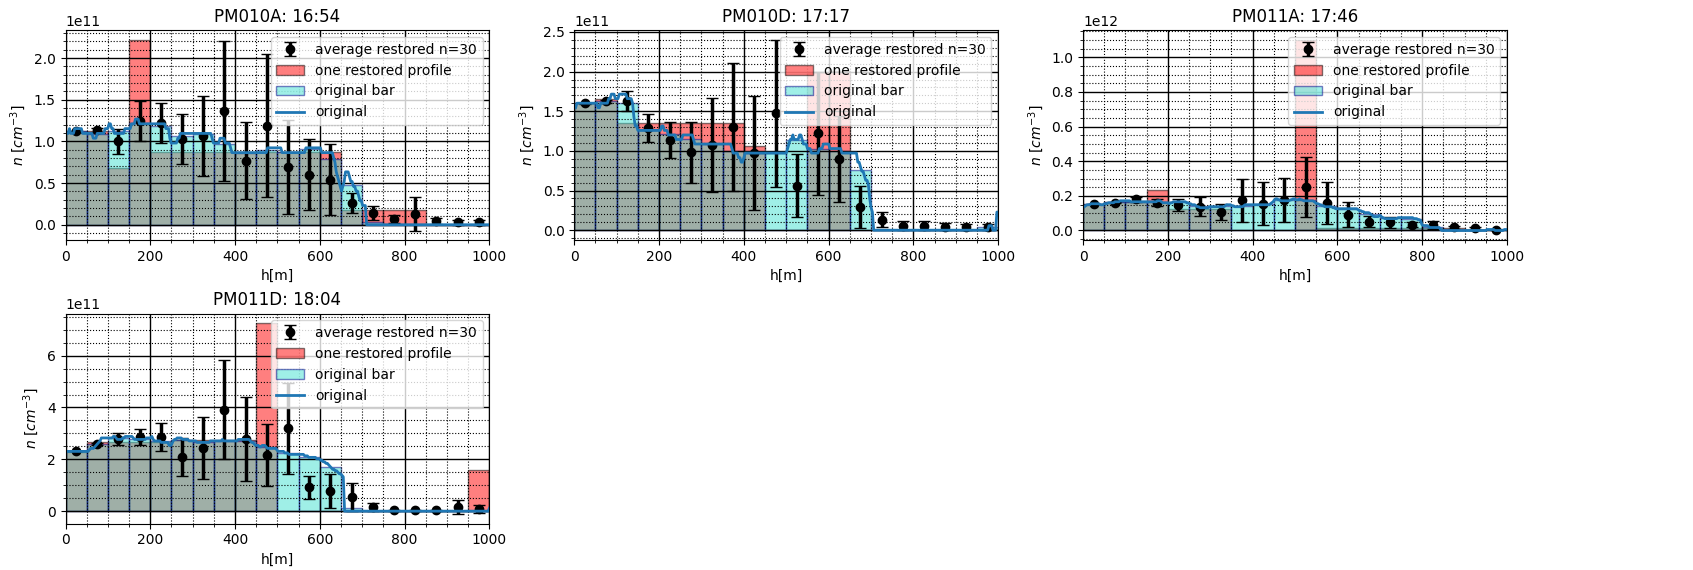
\includegraphics[width=180mm]{./pic/proff_2.png}
}
\caption{Результаты восстановления профилей при
$\text{szas}=60^{\circ}, \lambda_{NM}= 450\text{нм},
\text{albedo}=0.05, \nu_j \sim 
\mathcal{N}(0, (0.1 * 10^{15})^2)$.}
\label{proff_12}
\end{figure}
\clearpage
\begin{figure}[bh]
\noindent\centering{
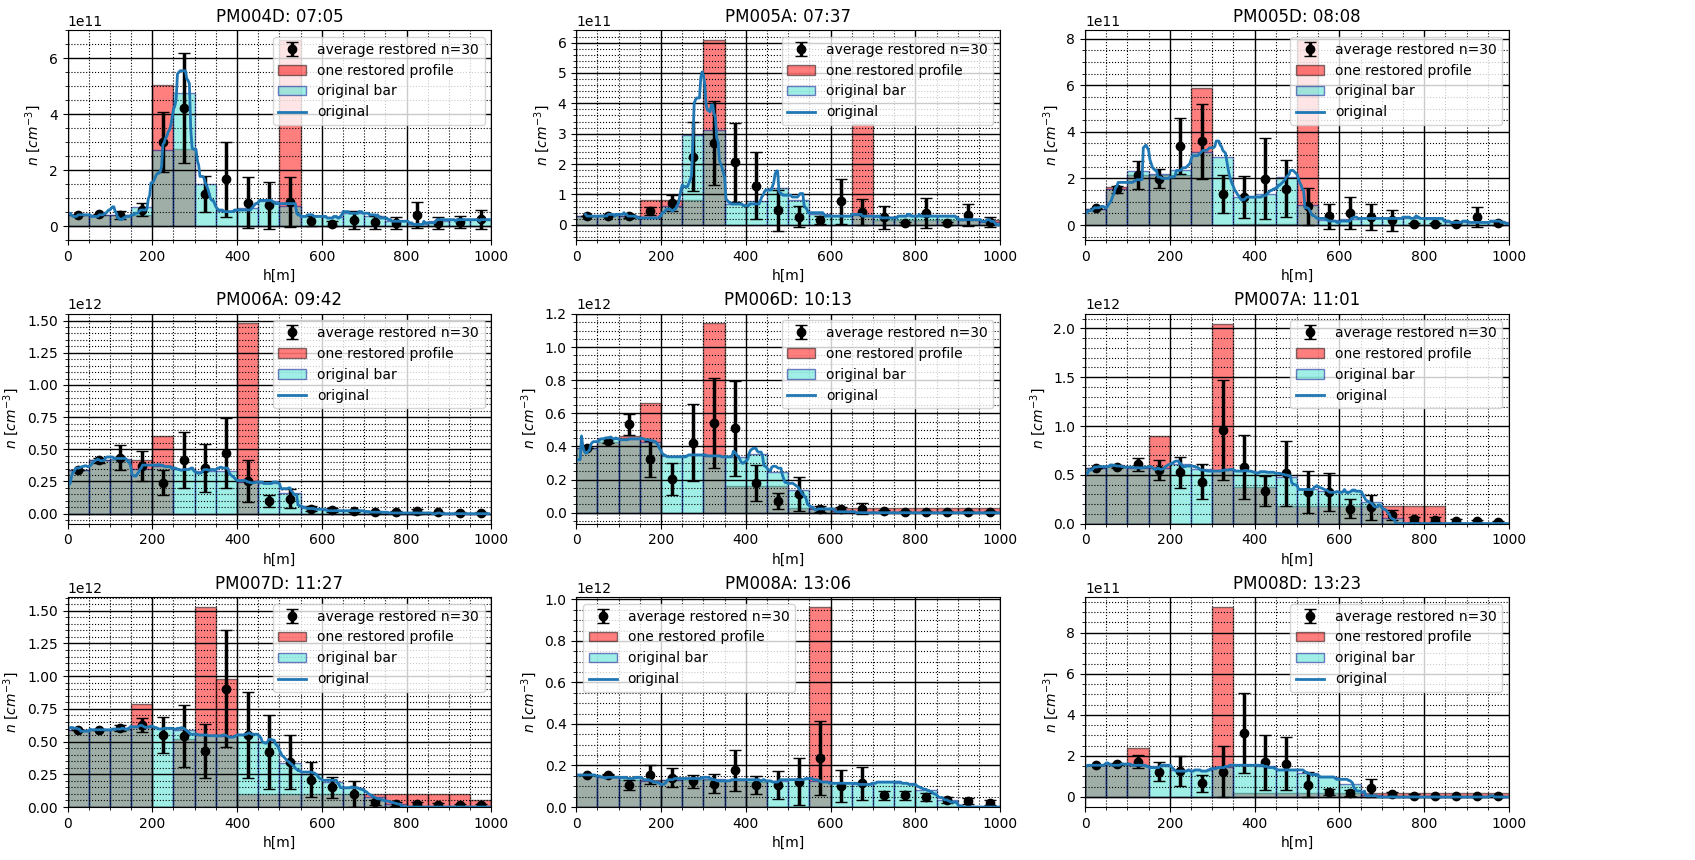
\includegraphics[width=180mm]{./pic/proff3_1.png}
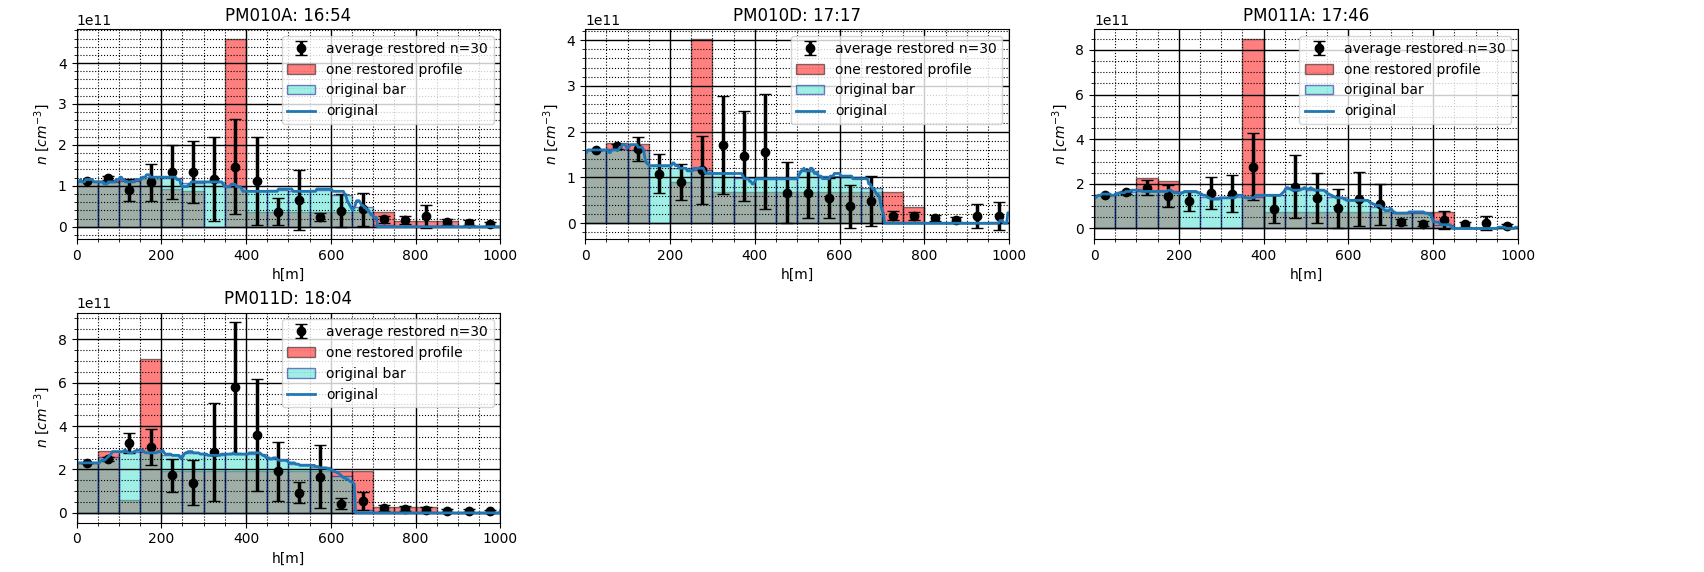
\includegraphics[width=180mm]{./pic/proff3_2.png}
}
\caption{Результаты восстановления профилей при
$\text{szas}=60^{\circ}, \lambda_{NM}= 450\text{нм},
\text{albedo}=0.05, \nu_j \sim 
\mathcal{N}(0, (0.3 * 10^{15})^2)$.}
\label{proff3_12}
\end{figure}
\clearpage
\section{Обсуждение результатов}
Видно, что исследуемый нами метод, решающий задачу вертикального
восстановления, является устойчивым за счет введения
дополнительных условий на унимодальность и неотрицательность,
и в целом может корректно описывать профили как с одним, так
и с двумя максимумами.
\nl
Метод достаточно чувствителен к уровню шума:
при его увеличении происходит линейное увеличение
ошибки(стандартного отклонения) при рассмотрении выборки из 
$30$-ти восстановленных профилей, 
что отражается в первую очередь на выборе параметра 
$c$($c_1, c_2, c_3$ в случае двух максимумов), 
отвечающий за положение максимума,
который выбирается по принципу минимизации невязки.
\nl
Сгенерировав модельные профили, состоящие из двух 
выраженных ступенек, можно качественно показать отличия
в восстановлении при требованиях унимодальности или 
термодальности\footnote{(От лат. нареч.) три} профиля.
\nl
На Рис.\ref{pic:threemode_12} видно, 
что, в предположении одного максимума проиходит сглаживание 
двух пиков при сохрании интегральной концентрации под ними.
В преположении двух максимумов(нижние $6$ графиков) 
пики восстанавливаются достаточно отчётливо. 
\begin{figure}[bh]
\noindent\centering{
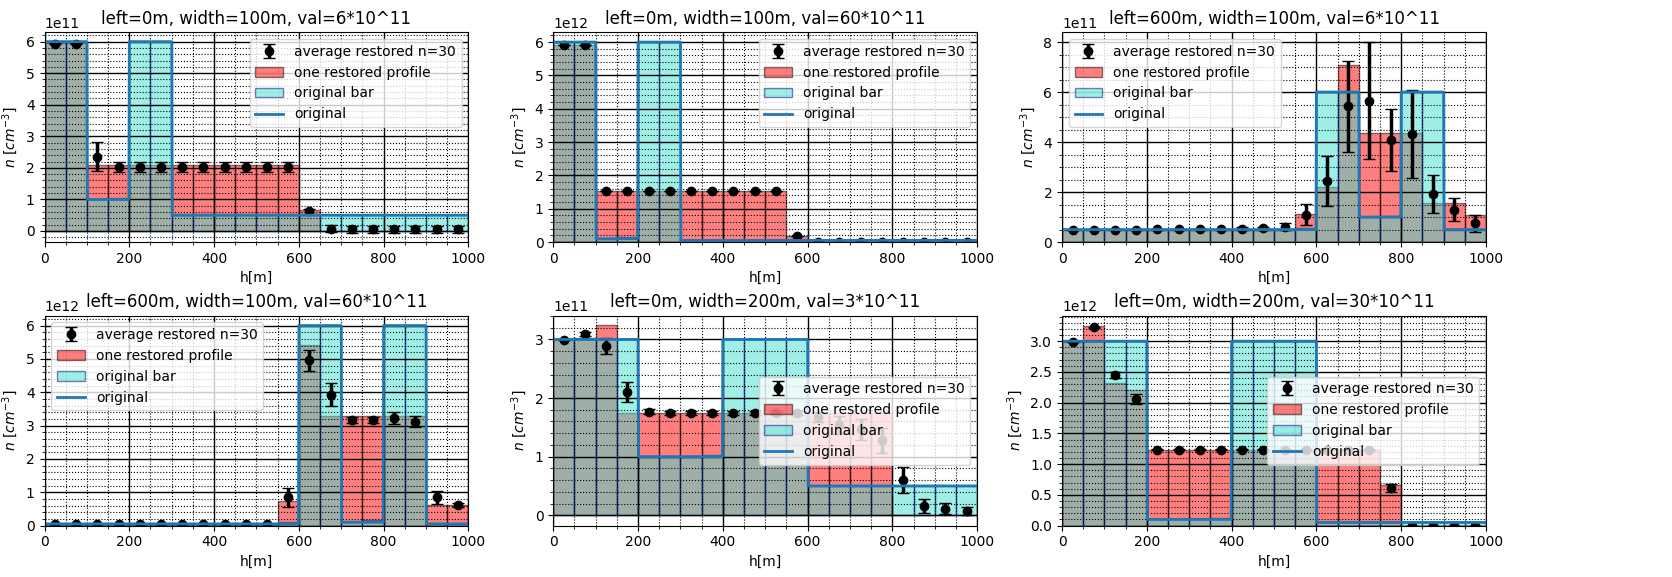
\includegraphics[width=180mm]{./pic/threemode_1.png}
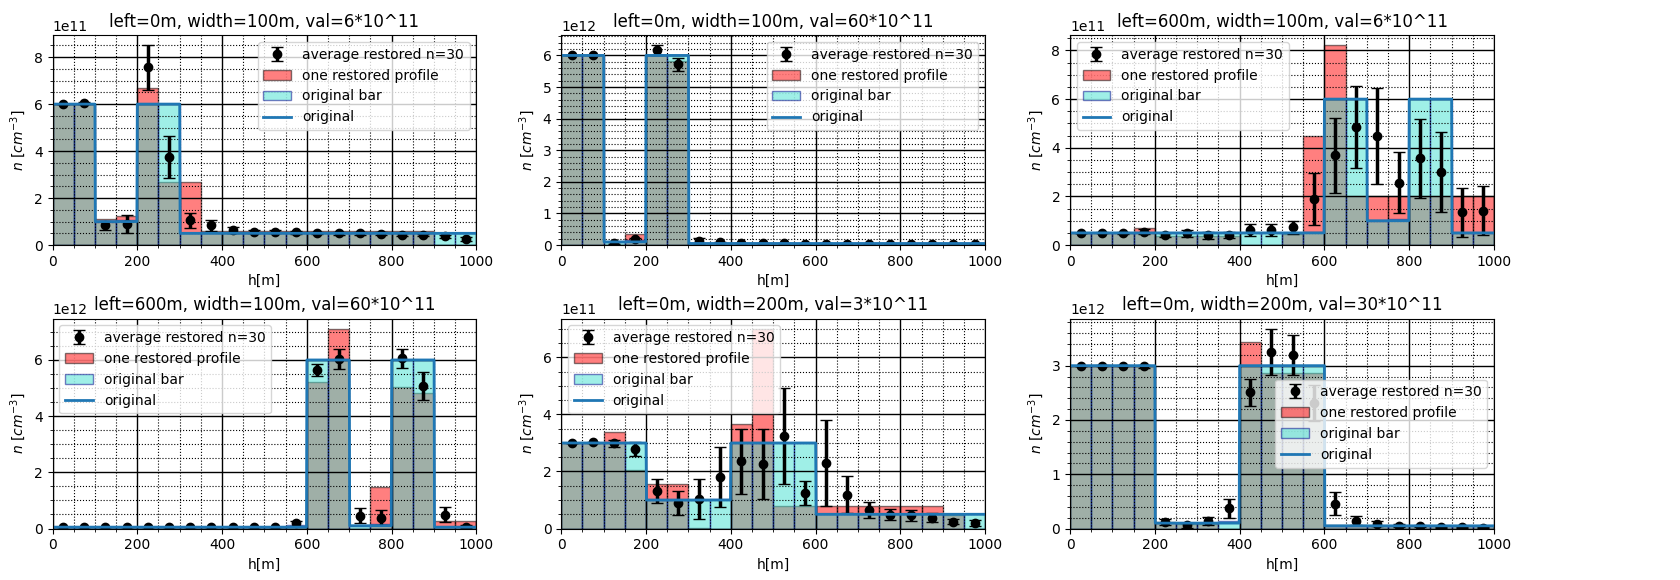
\includegraphics[width=180mm]{./pic/threemode_2.png}
}
\caption{Результаты восстановления модельных профилей при
$\text{szas}=60^{\circ}, \lambda_{NM}= 450\text{нм},
\text{albedo}=0.05, \nu_j \sim 
\mathcal{N}(0, (0.1 * 10^{15})^2)$.}
\label{pic:threemode_12}
\end{figure} 
\clearpage 
\section{Заключение}
В ходе работы была исследована возможность восстановления
профиля \no в атмосфере при помощи сведения обратной задачи к 
задаче линейного программирования при различных уровнях
зашумлённости сигнала и при учёте различного рода априорной
информации о форме профиля.
\nl 
В дальнейшем планируется усложнение модели и алгоритма 
путём продления восстанавливаемого профиля до $3-4\text{км}$,
переходом от дифференциальных наклонных толщ
$[dS(\theta) = S(\theta) - S(90^{\circ})]$, 
которые получаются в реальности к наклонным, добавлением
приземного измерения, оптимизацией измерения за 
счет перераспределения времени накопления сигнала между
различными углами.
\newpage
\addcontentsline{toc}{section}{Список используемой литературы}
\begin{thebibliography}{}
    \bibitem{litlink1}Friess, U. et al. Intercomparison of 
    MAX-DOAS vertical profile retrieval algorithms: 
    studies using synthetic data, Atmos. Meas. Tech., 12, 
    2155–2181, https://doi.org/10.5194/amt-12-2155-2019, 2019.
    \bibitem{litlink2}  О.В. Постыляков. Модель переноса 
    радиации в сферической атмосфере с расчетом послойных
    воздушных масс и некоторые ее приложения. 
    Известия РАН, ФАО, 2004, 40, №3, 314-329.
    \bibitem{litlink3}  G. Honninger, C. von Friedeburg
,U. Platt. Multi axis differential optical absorption
spectroscopy (MAX-DOAS). Atmos. Chem. Phys., 4, 231–254, 2004.
	\bibitem{litlink4} J. T. Pisano, I. Mckendry, D. G. Steyn 
and D. R. Hastie VERTICAL NITROGEN DIOXIDE AND OZONE
CONCENTRATIONS MEASURED FROM A TETHERED BALLOON IN THE LOWER
FRASER VALLEY // Atmospheric Environment Vol. 31, No.14, pp.
2071-2078, 1997
	\bibitem{litlink5} Udo Frie, Steffen Beirle, Leonardo
Alvarado Bonilla Intercomparison of MAX-DOAS vertical profile
retrieval algorithms: studies using synthetic data // Atmos.
Meas. Tech., 12, 2155–2181, 2019
	\bibitem{litlink6} A. Borovski, O. Postylyakov, A. Elokhov,
I. Bruchkovski Study of different operational modes of the 
IAP 2-port-DOAS instrument for atmospheric trace gases
investigation during CINDI-2 campaign basing on residual 
noise analysis
	\bibitem{litlink7} А.И.Чуличков Экстремальные задачи 1996
	\bibitem{litlink8} Ф.П. Васильев Методы оптимизации 2011
	\bibitem{litlink9} Хемди А. Таха Введение в исследование операций 2007
\end{thebibliography}
\end{document}




